\documentclass[table,aspectratio=169]{beamer}
%% Choose aspect ratio:
% [aspectratio=43]  % 4:3 (default)
% [aspectratio=169] % 16:9, wide

\usetheme[minimal, nofont, noheadline]{tugraz2018}
% \usetheme[iaik,]{tugraz2018}
%% Choose main theme variant:
% [standard]        % standard (default)
% [iaik]       % with institute's graphical acronym on the left
% [minimal]         % with reduced visuals

%% Choose your font style:
%                   % Helvetica (default for Corporate Design)
% [webfont]         % Source Sans Pro (as used on tugraz.at)
% [nofont]          % no font loaded - Computer Modern Sans

%% Choose your department's color instead of TU Graz tugred (optional):
% [arch]            % 
% [bau]             %
% [etit]            %
% [mbww]            %
% [tcvp]            %
% [mpug]            %
% [infbio]          %


\usepackage[utf8]{inputenc}
\usepackage[english]{babel}
%% Choose your language:
% [ngerman]   % German
% [english]   % English


%% Add your own packages, macros, etc.
\usepackage{xcolor, colortbl}
\usepackage{mathtools}
\usepackage{booktabs,nicematrix}
\usepackage{rotating}
\usepackage{listings}
\usepackage[style=alphabetic,backend=biber]{biblatex} % Bibliography
\addbibresource{\jobname.bib}                         % Bibliography
\usepackage{fontawesome}
\usepackage{filecontents}
\usepackage{mathrsfs}
\usepackage{amsmath}
\usepackage{setspace}
\usepackage{subcaption}
\usepackage{multirow}
\usepackage{bm}
\usepackage{pgfplots}
\usepackage[linesnumbered,ruled,vlined]{algorithm2e}
\usepackage{framed, color}

\usepackage{tikz}
\usepgfplotslibrary{external} % Library for externalization
\usetikzlibrary{calc, patterns, cipher, arrows.meta, shapes.geometric, positioning, decorations.pathreplacing, decorations.markings, decorations.pathmorphing}
\usepackage{skinny}
\usepackage{tugcolors}
\usepackage{skinnyzero} % definitions for figures: colors, etc
\setbeamersize
{
	text margin left=0.4cm,
	text margin right=0.4cm
}

%% Enter presentation metadata
\title{Cryptanalysis of \texttt{QARMAv2}}
\author{\underline{\textbf{Hosein Hadipour}} \and Yosuke Todo}
\date{FSE 2024 - Leuven, Belgium}
%\institute{IAIK}
\instituteurl{hsn.hadipour@gmail.com}

%% Logos
%\institutelogo{beamerthemetugraz/institute/IAIK}  % graphical acronym for [] theme (left margin)
% \additionallogo{figures/logo}  % additional institute/department logo (footline; optional)
% \logobar{Supported by: ...}  % sponsors (titlepage; optional)

%% Macros
\newcommand{\tikzmark}[1]{\tikz[overlay,remember picture] \node (#1) {};}
\newcommand{\pstabstyle}{\small\renewcommand{\tabcolsep}{3pt}}
%\newcommand{\KeysData}{Keys & Data}
%\newcommand{\KeysData}{\multicolumn{2}{c}{K $\times$ D}}
\newcommand{\KeysData}{K & D}

\newcommand{\smallmath}{\everydisplay{\fontsize{8pt}{10pt}\selectfont}}

%%% commands to represent CSP/COP variables/constraints%%%
\newcommand{\ax}{\texttt{AX}\xspace} %AX
\newcommand{\ay}{\texttt{AY}\xspace} %AY
\newcommand{\az}{\texttt{AZ}\xspace} %AZ
\newcommand{\dx}{\texttt{DX}\xspace} %DX
\newcommand{\dy}{\texttt{DY}\xspace} %DY
\newcommand{\dz}{\texttt{DZ}\xspace} %DZ

\newcommand{\axu}{\texttt{AXU}\xspace} %AXU
\newcommand{\ayu}{\texttt{AYU}\xspace} %AYU
\newcommand{\azu}{\texttt{AZU}\xspace} %AZU
\newcommand{\dxu}{\texttt{DXU}\xspace} %DXU
\newcommand{\dyu}{\texttt{DYU}\xspace} %DYU
\newcommand{\dzu}{\texttt{DZU}\xspace} %DZU
\newcommand{\lxu}{\texttt{LXU}\xspace} %LXU
\newcommand{\axl}{\texttt{AXL}\xspace} %AXL
\newcommand{\ayl}{\texttt{AYL}\xspace} %AYL
\newcommand{\azl}{\texttt{AZL}\xspace} %AZL
\newcommand{\dxl}{\texttt{DXL}\xspace} %DXL
\newcommand{\dyl}{\texttt{DYL}\xspace} %DYL
\newcommand{\dzl}{\texttt{DZL}\xspace} %DZL
\newcommand{\lxl}{\texttt{LXL}\xspace} %LXL
\newcommand{\astk}{\texttt{ASTK}\xspace} %ASTK

\newcommand{\D}{\texttt{D}\xspace} %Data complexity D[0], D[1]
\newcommand{\T}{\texttt{T}\xspace} %Time complexity T[0], T[1], T[2], T[3]
\newcommand{\W}{\texttt{W}\xspace} %hamming weight of IO differences
\newcommand{\C}{\texttt{C}\xspace} %c parameters c\In, c\Out
\newcommand{\s}{\texttt{c}\xspace} %s: cell size in our CP formulas
\newcommand{\z}{\texttt{z}\xspace} %z: number of tweakey paths in SKINNY

\newcommand{\cp}[1]{\textit{\texttt{#1}}\xspace} % CP x
\newcommand{\csp}{\textit{\texttt{CSP}}\xspace} % CSP problem
\newcommand{\cop}{\textit{\texttt{COP}}\xspace} % COP problem
\newcommand{\cpmodel}{\mathcal{M}\xspace} % CP model M
\newcommand{\cpvars}{\mathcal{M}.\texttt{var}\xspace} % CP variables
\newcommand{\cpcons}{\mathcal{M}.\texttt{con}\xspace} % CP constraints
\newcommand{\cpobj}{\mathcal{M}.\texttt{obj}\xspace} % CP objective
\newcommand{\booltoint}{\textit{\texttt{bool2int}}\xspace} % CP bool2int operator
\newcommand{\cpif}{\textit{\texttt{if}}\xspace} % CP If
\newcommand{\cpthen}{\textit{\texttt{then}}\xspace} % CP Then
\newcommand{\cpelse}{\textit{\texttt{else}}\xspace} % CP Else
\newcommand{\cpelseif}{\textit{\texttt{elseif}}\xspace} % CP Elseif
\newcommand{\cpendif}{\textit{\texttt{endif}}\xspace} % CP Endif

\newcommand{\cplink}{\textit{\texttt{Link}}\xspace} % CP Link
\newcommand{\cpxor}{\textit{\texttt{XOR}}\xspace} % CP XOR
\newcommand{\cpsbox}{\textit{\texttt{S-box}}\xspace} % CP S-box
\newcommand{\cpbranch}{\textit{\texttt{Branch}}\xspace} % CP Branching
\newcommand{\cpcopy}{\textit{\texttt{Copy}}\xspace} % Copy: equivalent to branching point
\newcommand{\cptrue}{\textit{\texttt{True}}\xspace} % CP True
\newcommand{\cpfalse}{\textit{\texttt{False}}\xspace} % CP False
\newcommand{\cpmin}{\textit{\texttt{min}}\xspace} % CP Min
\newcommand{\cpmdiff}{\textit{\texttt{Mdiff}}\xspace} % CP Mdiff
\newcommand{\cpminvdiff}{\textit{\texttt{Minvdiff}}\xspace} % CP Minvdiff

% notation for ID and figures
\newcommand{\In}{_{\textsc{b}}} % input difference of Ei (initial key-recovery rounds)
\newcommand{\Out}{_{\textsc{f}}} % output difference of Eo (final key-recovery rounds)
\newcommand{\Up}{_{\textsc{u}}} % input difference of Eu (initial distinguisher rounds)
\newcommand{\Low}{_{\textsc{l}}} % output difference of El (final distinguisher rounds)
\newcommand{\Dist}{_{\textsc{d}}} % distinguisher rounds Eu, El (middle)
\newcommand{\KB}{_{\textsc{KB}}} % Key-Bridging
\newcommand{\GD}{_{\textsc{GD}}} % Guess-and-Determine
\newcommand{\DP}{_{\textsc{DP}}} % Difference Propagation
\newcommand{\Off}{_{\text{off}}} % offset for round counter in Eu, El, and Ef
\newcommand{\Tot}{_\textit{Tot}}
\newcommand{\STK}{\textit{STK}}
\newcommand{\ETK}{\textit{ETK}}
\newcommand{\TK}{\textit{TK}}
\newcommand{\lane}{\textit{Lane}}
\newcommand{\cs}{c} % indicates the cell size in the main body
\newcommand{\as}{m} % indicates the state array size in the main body
\newcommand{\Rinit}{\textbf{r}_{\textbf{i}}} % Rinit for ForkSKINNY: the number of rounds before fork
\newcommand{\Rzero}{\textbf{r}_{\textsc{0}}} % R0 for ForkSKINNY: the length of C0 branch
\newcommand{\Rone}{\textbf{r}_{\textsc{1}}} % R1 for ForkSKINNY: the length of C1 branch
\newcommand{\bis}{\text{--}}

%%% format of the codes %%%
\lstdefinelanguage{Sage}[]{Python}{morekeywords={True,False,sage,cdef,cpdef,ctypedef,self, elseif, endif},sensitive=true}

\lstdefinestyle{mystyle}{
  backgroundcolor=\color{backcolour},
  commentstyle=\color{codegreen},
  keywordstyle={\color{magenta}\bfseries},
  numberstyle=\tiny\color{codegray},
  stringstyle=\color{codepurple},
  basicstyle=\ttfamily\footnotesize,
  breakatwhitespace=false,
  breaklines=true,
  captionpos=b,
  keepspaces=true,
  numbers=left,
  numbersep=5pt,
  showspaces=false,
  showstringspaces=false,
  showtabs=false,
  tabsize=2
}
\lstset{style=mystyle, language=Sage}
\definecolor{codegreen}{rgb}{0,0.6,0}
\definecolor{codegray}{rgb}{0.5,0.5,0.5}
\definecolor{codepurple}{rgb}{0.58,0,0.82}
\definecolor{backcolour}{rgb}{0.95,0.95,0.92}

\makeatletter
\NewDocumentCommand{\DrawBox}{s O{}}{%
    \tikz[overlay,remember picture]{
    \IfBooleanTF{#1}{%
        \coordinate (RightPoint) at ($(left |- right)+(\linewidth-\labelsep-\labelwidth,0.0)$);
    }{%
        \coordinate (RightPoint) at (right.east);
    }%
    \draw[red,#2]
      ($(left)+(-0.2em,0.9em)$) rectangle
      ($(RightPoint)+(0.2em,-0.3em)$);}
}

\NewDocumentCommand{\DrawBoxWide}{s O{}}{%
    \tikz[overlay,remember picture]{
    \IfBooleanTF{#1}{%
        \coordinate (RightPoint) at ($(left |- right)+(\linewidth-\labelsep-\labelwidth,0.0)$);
    }{%
        \coordinate (RightPoint) at (right.east);
    }%
    \draw[red,#2]
      ($(left)+(-\labelwidth,0.9em)$) rectangle
      ($(RightPoint)+(0.2em,-0.3em)$);}
}

\def\rowcolor{\noalign{\ifnum0=`}\fi\bmr@rowcolor}
\newcommand<>{\bmr@rowcolor}{%
    \alt#1%
        {\global\let\CT@do@color\CT@@do@color\@ifnextchar[\CT@rowa\CT@rowb}% 
        {\ifnum0=`{\fi}\@gooble@rowcolor}% 
}
\newcommand{\@gooble@rowcolor}[2][]{\@gooble@rowcolor@}
\newcommand{\@gooble@rowcolor@}[1][]{\@gooble@rowcolor@@}
\newcommand{\@gooble@rowcolor@@}[1][]{\ignorespaces}

%%%%%%%%%%%%%%%%%%%%%%%%%%%%%%%%%%%%%%%%%%%%%%%%%%%%%%%%%%%%%%%%%%%%%%%%
% For Partial-sum example on AES
\colorlet{act}{tugyellow}
\colorlet{con}{white}
\colorlet{bal}{colB}
\newcommand{\PSfont}{\footnotesize}
\newcommand{\PScale}{.88}
\newcommand{\iAct}[1]{\Fill[act]{#1}\Cell{#1}{\color{white}\PSfont A}}
\newcommand{\iBal}[1]{\Fill[bal]{#1}\Cell{#1}{\color{white}\PSfont B}}
\newcommand{\iCon}[1]{\Fill[con]{#1}\Cell{#1}{\color{gray}\PSfont C}}
\newcommand{\iStep}[2]{\Fill[tugblue]{#1}\Cell{#1}{\color{white}\PSfont\texttt #2}}
\newcommand{\iKey}[2]{\Fill[tuggreen]{#1}\Cell{#1}{\color{white}\PSfont\texttt #2}}
\newcommand{\iPartial}[2]{\Fill[tugyellow]{#1}\Cell{#1}{\color{white}\PSfont\texttt #2}}

\newcommand{\SingleCell}[1]{
  \tikz[stateopts]{ %, rounded corners=2pt
    \draw (.5,-.5) coordinate (s);
    #1
  }  
}

\newcommand{\PartialSumStepInit}{
  \tikz[yscale=\PScale]{
    \foreach \i/\s in {0/1,1/1,2/2,3/3} {
      \ifcase \i
        \draw ++(\i*.5+1,0) node[inner sep=0pt] (c\i) {\SingleCell{\iStep{s}{\s}}};
      \or
        \draw ++(\i*.5+1,0) node[inner sep=0pt] (c\i) {\SingleCell{\iStep{s}{\s}}};
      \else
        \draw ++(\i*.5+1,0) node[inner sep=0pt, opacity=0.5] (c\i) {\SingleCell{\iStep{s}{\s}}};
      \fi
    }

    \foreach \i/\in/\s in {0/0/1,1/1/1} {
      \draw (c\in) ++(0,-.5-\i*.35) coordinate[xor] (xorc\i);
      \draw (c0) ++(-\in*.5-.5, 0) node[inner sep=0pt] (k\i) {\SingleCell{\iKey{s}{\s}}};
      \draw (c\in.south) ++(0,-1.3) node[sbox,inner sep=2pt] (sbox\in) {$\mathcal{S}_{\i}$};

      \draw[->, rounded corners=2pt] (c\in.south) -- (xorc\in.north);
      \draw[->, rounded corners=2pt] (k\in.south) |- (xorc\in.west);

      \draw[->, rounded corners=2pt] (xorc\in) -- (sbox\in);
    }

    \draw (sbox1) ++(0,-.5) coordinate[xor] (xors);

    \draw[->, rounded corners=2pt] (sbox1) -- (xors);
    \draw[->, rounded corners=2pt] (sbox0) |- (xors);

    \draw (c2 |- xors) ++(0,-.5) node[sbox, minimum width=3.0cm, inner sep=2pt] (count) {\texttt{count}};

    \draw[->, rounded corners=2pt] (xors.south) -- (xors |- count.north);
    \draw[->, rounded corners=2pt] (c2.south) -- (c2 |- count.north);
    \draw[->, rounded corners=2pt] (c3.south) -- (c3 |- count.north);

    \draw[->, rounded corners=2pt] (xors |- count.south) -- ++(0,-.2);
    \draw[->, rounded corners=2pt] (c2 |- count.south) -- ++(0,-.2);
    \draw[->, rounded corners=2pt] (c3 |- count.south) -- ++(0,-.2);
  }
}

\newcommand{\PartialSumStepTwo}{
  \tikz[yscale=\PScale]{
    \draw node[inner sep=0pt, opacity=0.5] (k1) {\SingleCell{\iKey{s}{1}}}
    ++(.5, 0) node[inner sep=0pt, opacity=0.5] (k2) {\SingleCell{\iKey{s}{1}}}
    ++(.5, 0) node[inner sep=0pt] (k) {\SingleCell{\iKey{s}{2}}}
    ++(.5,0) node[inner sep=0pt] (c1) {\SingleCell{\iPartial{s}{2}}}
    ++(.5,0) node[inner sep=0pt] (c2) {\SingleCell{\iStep{s}{2}}}
    ++(.5,0) node[inner sep=0pt, opacity=0.5] (c3) {\SingleCell{\iStep{s}{3}}};


    \draw (c2) ++(0,-.5) coordinate[xor] (xorc);

    \draw (c2.south) ++(0,-.8) node[sbox,inner sep=2pt] (sbox) {$\mathcal{S}_{2}$};

    \draw[->, rounded corners=2pt] (c2.south) -- (xorc.north);
    \draw[->, rounded corners=2pt] (k.south) |- (xorc.west);

    \draw[->, rounded corners=2pt] (xorc) -- (sbox);

    \draw (sbox) ++(0,-.5) coordinate[xor] (xors);

    \draw[->, rounded corners=2pt] (sbox) -- (xors);
    \draw[->, rounded corners=2pt] (c2.south) ++(-.5,0) -- ++(0,-1.3) -- (xors);

    \draw (c2 |- xors) ++(.25,-.5) node[sbox, minimum width=2.15cm, inner sep=2pt] (count) {\texttt{count}};

    \draw[->, rounded corners=2pt] (xors.south) -- (xors |- count.north);
    \draw[->, rounded corners=2pt] (c3.south) -- (c3 |- count.north);

    \draw[->, rounded corners=2pt] (xors |- count.south) -- ++(0,-.2);
    \draw[->, rounded corners=2pt] (c3 |- count.south) -- ++(0,-.2);
  }  
}

\newcommand{\PartialSumStepThree}{
  \tikz[yscale=\PScale]{
    \draw node[inner sep=0pt, opacity=0.5] (k1) {\SingleCell{\iKey{s}{1}}}
    ++(.5, 0) node[inner sep=0pt, opacity=0.5] (k2) {\SingleCell{\iKey{s}{1}}}
    ++(.5, 0) node[inner sep=0pt, opacity=0.5] (k3) {\SingleCell{\iKey{s}{2}}}
    ++(.5, 0) node[inner sep=0pt] (k) {\SingleCell{\iKey{s}{3}}}
    ++(.5,0) node[inner sep=0pt] (c1) {\SingleCell{\iPartial{s}{3}}}
    ++(.5,0) node[inner sep=0pt] (c2) {\SingleCell{\iStep{s}{3}}};

    \draw (c2) ++(0,-.5) coordinate[xor] (xorc);

    \draw (c2.south) ++(0,-.8) node[sbox,inner sep=2pt] (sbox) {$\mathcal{S}_{3}$};

    \draw[->, rounded corners=2pt] (c2.south) -- (xorc.north);
    \draw[->, rounded corners=2pt] (k.south) |- (xorc.west);

    \draw[->, rounded corners=2pt] (xorc) -- (sbox);

    \draw (sbox) ++(0,-.5) coordinate[xor] (xors);

    \draw[->, rounded corners=2pt] (sbox) -- (xors);
    \draw[->, rounded corners=2pt] (c2.south) ++(-.5,0) -- ++(0,-1.3) -- (xors);

    \draw (xors) ++(0,-.5) node[sbox, minimum width=1.3cm, inner sep=2pt] (count) {\texttt{count}};

    \draw[->, rounded corners=2pt] (xors.south) -- (xors |- count.north);

    \draw[->, rounded corners=2pt] (xors |- count.south) -- ++(0,-.2);
  }  
}

\newcommand{\PartialSumStepFinal}{
  \tikz[remember picture,yscale=\PScale]{
    \draw node[inner sep=0pt, opacity=0.5] (k1) {\SingleCell{\iKey{s}{1}}}
    ++(.5, 0) node[inner sep=0pt, opacity=0.5] (k2) {\SingleCell{\iKey{s}{1}}}
    ++(.5, 0) node[inner sep=0pt, opacity=0.5] (k3) {\SingleCell{\iKey{s}{2}}}
    ++(.5, 0) node[inner sep=0pt, opacity=0.5] (k3) {\SingleCell{\iKey{s}{3}}}
    ++(.5, 0) node[inner sep=0pt] (k) {\SingleCell{\iKey{s}{4}}}
    ++(.5,0) node[inner sep=0pt] (c) {\SingleCell{\iPartial{s}{4}}};

    \draw (c) ++(0,-.5) coordinate[xor] (xorc);
    \draw (c.south) ++(0,-.8) node[sbox, color=white, minimum width=1.3cm, inner sep=2pt] (dummy) {\texttt{count}};
    \draw (c.south) ++(0,-.8) node[sbox,inner sep=2pt] (sbox) {$\mathcal{S}^{-1}$};

    \draw[->, rounded corners=2pt] (c.south) -- (xorc.north);
    \draw[->, rounded corners=2pt] (k.south) |- (xorc.west);

    \draw[->, rounded corners=2pt] (xorc) -- (sbox);
  } 
}

%%%%%%%%%%%%%%%%%%%%%%%%%%%%%%%%%%%%%%%%%%%%%%%%%%%%%%%%%%%%%%%%%%%%%%%%

\newcommand{\sparen}{\vspace*{-.3cm}}


\makeatother

\begin{document}

\begin{frame}[plain]
  \maketitle
\end{frame}

\begin{frame}{Motivation and Our Contributions}
\begin{itemize}
  \item<1->[\faBinoculars] Motivation
  \begin{itemize}
    \item[\faCheckCircleO] Sheding more light on the security of \texttt{QARMAv2} against cryptanalysis.
  \end{itemize}
  \item<2->[\faDiamond] Contributions
  \begin{itemize}
    \item<2->[\faCheckCircle] Proposing a new CP-based tool to search for intergal distinguishers of tweakable block ciphers following the \texttt{TWEAKEY} framework.
    \item<2->[\faCheckCircle] Providing the first concrete key recovery attack against three main variants of \texttt{QARMAv2}. 
  \end{itemize}
\end{itemize}
\end{frame}

\section*{}
\begin{frame}{Outline}
  \tableofcontents
\end{frame}

%%%%%%%%%%%%%%%%%%%%%%%%%%%%%%%%%%%%%%%%%%%%%%%%%%%%%%%%%%%%%%%%%%%%%%%%%%%%%%%
%%%%%%%%%%%%%%%%%%%%%%%%%%%%%%%%%%%%%%%%%%%%%%%%%%%%%%%%%%%%%%%%%%%%%%%%%%%%%%%
\section{Background and Specification of \texttt{QARMAv2}}
\sectionheader[\huge\color{tug}\faBook]{Background and Specification of \texttt{QARMAv2}}

%%%%%%%%%%%%%%%%%%%%%%%%%%%%%%%%%%%%%%%%%%%%%%%%%%%%%%%%%%%%%%%%%%%%%%%%%%%%%%%
\begin{frame}{\texttt{QARMAv2} Family of Tweakable Block Ciphers \cite{cryptoeprint_qarmav2}}
\vspace{-0.7cm}
\begin{columns}
\column[c]{0.25\textwidth}
\begin{figure}
  \centering
  \begin{subfigure}[c]{0.2\textwidth}
  \scalebox{0.6}{
  \begin{tikzpicture}[cellopts/.append style={font=\tiny}]
    \node[state, rounded corners=2pt] (X) at (0,0) {\MatrixState{%
          \Cell{s0} {\ttfamily 0}\Cell{s1} {\ttfamily 1}\Cell{s2} {\ttfamily 2}\Cell{s3} {\ttfamily 3}
          \Cell{s4} {\ttfamily 4}\Cell{s5} {\ttfamily 5}\Cell{s6} {\ttfamily 6}\Cell{s7} {\ttfamily 7}
          \Cell{s8}{\ttfamily 8}\Cell{s9}{\ttfamily 9}\Cell{s10}{\ttfamily a}\Cell{s11}{\ttfamily b}
          \Cell{s12}{\ttfamily c}\Cell{s13}{\ttfamily d}\Cell{s14}{\ttfamily e}\Cell{s15}{\ttfamily f}}};
    \node[state, rounded corners=2pt] (TX) at (2.5,0) {\MatrixState{%
          \Cell{s0} {\ttfamily 0}\Cell{s1} {\ttfamily b}\Cell{s2} {\ttfamily 6}\Cell{s3} {\ttfamily d}
          \Cell{s4} {\ttfamily a}\Cell{s5} {\ttfamily 1}\Cell{s6} {\ttfamily c}\Cell{s7} {\ttfamily 7}
          \Cell{s8} {\ttfamily 5}\Cell{s9} {\ttfamily e}\Cell{s10}{\ttfamily 3}\Cell{s11}{\ttfamily 8}
          \Cell{s12}{\ttfamily f}\Cell{s13}{\ttfamily 4}\Cell{s14}{\ttfamily 9}\Cell{s15}{\ttfamily 2}}};
  
    \draw[->] (X) -- node[above] {$\tau$} (TX);
    \draw (X.south) node[below] {$X$};
    \draw (TX.south) node[below] {$\tau(X)$};
  \end{tikzpicture}}
  \end{subfigure}
  \vskip 0.1cm
  \begin{subfigure}[c]{0.2\textwidth}
  \centering
  \scalebox{0.6}{
  \begin{tikzpicture}[cellopts/.append style={font=\tiny}]
    \node[state, rounded corners=2pt] (X) at (0,0) {\MatrixState{%
          \Cell{s0} {\ttfamily 0}\Cell{s1} {\ttfamily 1}\Cell{s2} {\ttfamily 2}\Cell{s3} {\ttfamily 3}
          \Cell{s4} {\ttfamily 4}\Cell{s5} {\ttfamily 5}\Cell{s6} {\ttfamily 6}\Cell{s7} {\ttfamily 7}
          \Cell{s8}{\ttfamily 8}\Cell{s9}{\ttfamily 9}\Cell{s10}{\ttfamily a}\Cell{s11}{\ttfamily b}
          \Cell{s12}{\ttfamily c}\Cell{s13}{\ttfamily d}\Cell{s14}{\ttfamily e}\Cell{s15}{\ttfamily f}}};
    \node[state, rounded corners=2pt] (TX) at (2.5,0) {\MatrixState{%
          \Cell{s0} {\ttfamily 1}\Cell{s1} {\ttfamily a}\Cell{s2} {\ttfamily e}\Cell{s3} {\ttfamily 6}
          \Cell{s4} {\ttfamily 2}\Cell{s5} {\ttfamily 9}\Cell{s6} {\ttfamily d}\Cell{s7} {\ttfamily 5}
          \Cell{s8} {\ttfamily 0}\Cell{s9} {\ttfamily 8}\Cell{s10}{\ttfamily c}\Cell{s11}{\ttfamily 4}
          \Cell{s12}{\ttfamily 3}\Cell{s13}{\ttfamily b}\Cell{s14}{\ttfamily f}\Cell{s15}{\ttfamily 7}}};
    \draw[->] (X) -- node[above] {$\varphi$} (TX);
    \draw (X.south) node[below] {$T$};
    \draw (TX.south) node[below] {$\varphi(T)$};
  \end{tikzpicture}}  
  \end{subfigure}
  \vskip 0.1cm
  \begin{subfigure}[c]{0.2\textwidth}
    \centering
    \scalebox{0.6}{
    \begin{tikzpicture}[cellopts/.append style={font=\tiny}]
      \node[state, rounded corners=2pt] (X1) at (0,0) {\MatrixState{%
            \Cell{s0} {\ttfamily 0}\Cell{s1} {\ttfamily 1}\Cell{s2} {\ttfamily 2}\Cell{s3} {\ttfamily 3}
            \Cell{s4} {\ttfamily 4}\Cell{s5} {\ttfamily 5}\Cell{s6} {\ttfamily 6}\Cell{s7} {\ttfamily 7}
            \Cell{s8}{\ttfamily 8}\Cell{s9}{\ttfamily 9}\Cell{s10}{\ttfamily 10}\Cell{s11}{\ttfamily 11}
            \Cell{s12}{\ttfamily 12}\Cell{s13}{\ttfamily 13}\Cell{s14}{\ttfamily 14}\Cell{s15}{\ttfamily 15}}};
      \node[state, rounded corners=2pt] (X2) at (0, -1.21) {\MatrixState{%
            \Cell{s0} {\ttfamily 16}\Cell{s1} {\ttfamily 17}\Cell{s2} {\ttfamily 18}\Cell{s3} {\ttfamily 19}
            \Cell{s4} {\ttfamily 20}\Cell{s5} {\ttfamily 21}\Cell{s6} {\ttfamily 22}\Cell{s7} {\ttfamily 23}
            \Cell{s8}{\ttfamily 24}\Cell{s9}{\ttfamily 25}\Cell{s10}{\ttfamily 26}\Cell{s11}{\ttfamily 27}
            \Cell{s12}{\ttfamily 28}\Cell{s13}{\ttfamily 29}\Cell{s14}{\ttfamily 30}\Cell{s15}{\ttfamily 31}}};
      \node[state, rounded corners=2pt] (TX1) at (2.5,0) {\MatrixState{%
            \Cell{s0} {\ttfamily 1}\Cell{s1} {\ttfamily 10}\Cell{s2} {\ttfamily 14}\Cell{s3} {\ttfamily 22}
            \Cell{s4} {\ttfamily 18}\Cell{s5} {\ttfamily 25}\Cell{s6} {\ttfamily 29}\Cell{s7} {\ttfamily21}
            \Cell{s8} {\ttfamily 0}\Cell{s9} {\ttfamily 8}\Cell{s10}{\ttfamily 12}\Cell{s11}{\ttfamily 4}
            \Cell{s12}{\ttfamily 19}\Cell{s13}{\ttfamily 27}\Cell{s14}{\ttfamily 31}\Cell{s15}{\ttfamily 23}}};
      \node[state, rounded corners=2pt] (TX2) at (2.5,-1.21) {\MatrixState{%
            \Cell{s0} {\ttfamily 17}\Cell{s1} {\ttfamily 26}\Cell{s2} {\ttfamily 30}\Cell{s3} {\ttfamily 6}
            \Cell{s4} {\ttfamily 2}\Cell{s5} {\ttfamily 9}\Cell{s6} {\ttfamily 13}\Cell{s7} {\ttfamily 5}
            \Cell{s8} {\ttfamily 16}\Cell{s9} {\ttfamily 24}\Cell{s10}{\ttfamily 28}\Cell{s11}{\ttfamily 20}
            \Cell{s12}{\ttfamily 3}\Cell{s13}{\ttfamily 11}\Cell{s14}{\ttfamily 15}\Cell{s15}{\ttfamily 7}}};
      \draw[->] ($(X1.east)!.5!(X2.east)$) -- node[above] {$\varphi$} ($(TX1.west)!.5!(TX2.west)$);
      \draw (X2.south) node[below] {$T$};
      \draw (TX2.south) node[below] {$\varphi(T)$};
    \end{tikzpicture}} 
  \end{subfigure}
  \vskip 0.01cm
  \begin{subfigure}[c]{0.2\textwidth}
    \centering
    \bgroup\fontsize{5}{6}\selectfont
    \begin{align*}
      M\!\coloneqq\!&\begin{pmatrix}
        0 & \rho & \rho^2 & \rho^3\\
        \rho^3 & 0 & \rho & \rho^2\\
        \rho^2 & \rho^3 & 0 & \rho\\
        \rho & \rho^2 & \rho^3 & 0
      \end{pmatrix}\\
      \rho \in& \mathbb{F}_{2}^{4}, \rho^{4} = 1
    \end{align*}
    \egroup
  \end{subfigure}
\end{figure}
\column[c]{0.75\textwidth}
\begin{figure}
  \centering
  \begin{subfigure}{0.5\textwidth} % Specify the width for the first subfigure
    \centering
    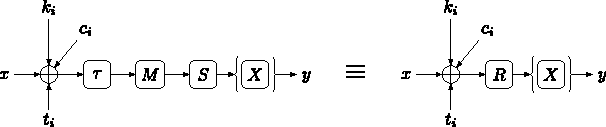
\includegraphics[width=1.1\textwidth]{./figures/qarmav2_full_round.pdf}
  \end{subfigure}
  \vskip 0.2cm
  % \vspace{0.3cm}
  \begin{subfigure}{0.9\textwidth} % Specify the width for the second subfigure
    \centering
    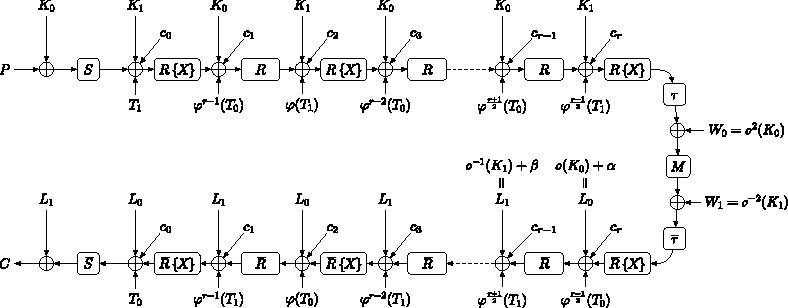
\includegraphics[width=1\textwidth]{./figures/qarmav2_odd_rounds.pdf}
  \end{subfigure}
\end{figure}
\end{columns}
\end{frame}

%%%%%%%%%%%%%%%%%%%%%%%%%%%%%%%%%%%%%%%%%%%%%%%%%%%%%%%%%%%%%%%%%%%%%%%%%%%%%%%
\begin{frame}{Security Parameters}
\sparen
\begin{table}
  \centering
  \begin{subtable}{\textwidth}
  \centering
  \caption*{Parameters of \texttt{QARMAv2} with two tweak blocks ($\mathscr{T} = 2$).}
  \resizebox{0.6\textwidth}{!}{
  \begin{tabular}{lcccccc}
    \toprule
    Version & Block size $(b)$ & Key Size $(s)$ & $r$ & \#Rounds & Time & Data\\
    \hline
    \texttt{QARMAv2}-64-128 & 64 & 128 & 9 & 20 & $2^{128 - \varepsilon}$ & $2^{56}$\\
    \midrule    
    \texttt{QARMAv2}-128-128 & 128 & 128 & 11 & 24 & $2^{128 - \varepsilon}$ & $2^{80}$\\
    \midrule
    \texttt{QARMAv2}-128-192 & 128 & 192 & 13 & 28 & $2^{192 - \varepsilon}$ & $2^{80}$\\
    \midrule
    \texttt{QARMAv2}-128-256 & 128 & 256 & 15 & 32 & $2^{256 - \varepsilon}$ & $2^{80}$\\
    \bottomrule
  \end{tabular}}
  \end{subtable}
  \bigskip
  \begin{subtable}{\textwidth}
  \centering
  \caption*{Parameters of \texttt{QARMAv2} with a single tweak block ($\mathscr{T} = 1$).}
  \resizebox{0.6\textwidth}{!}{
  \begin{tabular}{lcccccc}    
    \toprule
    Version & Block size $(b)$ & Key Size $(s)$ & $r$ & \#Rounds & Time & Data\\
    \hline
    \texttt{QARMAv2}-64-128 & 64 & 128 & 7 & 16 & $2^{128 - \varepsilon}$ & $2^{56}$\\
    \midrule    
    \texttt{QARMAv2}-128-128 & 128 & 128 & 9 & 20 & $2^{128 - \varepsilon}$ & $2^{80}$\\
    \midrule
    \texttt{QARMAv2}-128-192 & 128 & 192 & 11 & 24 & $2^{192 - \varepsilon}$ & $2^{80}$\\
    \midrule
    \texttt{QARMAv2}-128-256 & 128 & 256 & 13 & 28 & $2^{256 - \varepsilon}$ & $2^{80}$\\
    \bottomrule
  \end{tabular}}
  \end{subtable}
\end{table}
\end{frame}

%%%%%%%%%%%%%%%%%%%%%%%%%%%%%%%%%%%%%%%%%%%%%%%%%%%%%%%%%%%%%%%%%%%%%%%%%%%%%%%
\begin{frame}{Designers' Analyses \cite{cryptoeprint_qarmav2}}
\begin{figure}
\centering
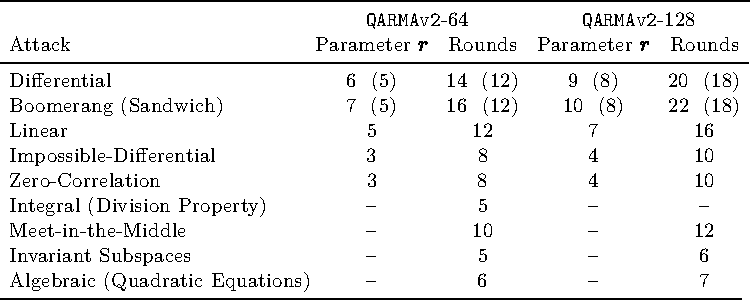
\includegraphics[width=\textwidth]{./figures/attacks_table.pdf}
\end{figure}
\end{frame}

%%%%%%%%%%%%%%%%%%%%%%%%%%%%%%%%%%%%%%%%%%%%%%%%%%%%%%%%%%%%%%%%%%%%%%%%%%%%%%%
\begin{frame}{Integral and Zero-Correlation (ZC) Distinguishers}
\begin{itemize}
\small
\item Integral attacks \cite{hod_discrete_derivatives_lai1994higher, square_fse_DaemenKR97}
\item ZC attacks \cite{dcc_BogdanovR14}
\end{itemize}
\begin{block}{Link Between ZC and Integral Distinguishers \textcolor{white}{\cite{crypto_SunLRLCWAL15}}}
Let $F:\mathbb{F}_{2}^{n}\rightarrow \mathbb{F}_{2}^{n}$ be a vectorial Boolean function. 
Assume $A$ is a subspace of $\mathbb{F}_{2}^{n}$ and $\beta\in \mathbb{F}_{2}^{n}\setminus \{0\}$
such that $(\alpha, \beta)$ is a ZC approximation for any $\alpha \in A$. 
Then, for any $\lambda \in \mathbb{F}_{2}^{n}$, $\left\langle \beta, F(x + \lambda)\right\rangle$ is balanced over the set
\[A^{\bot} = \{x \in \mathbb{F}_{2}^{n}~|~ \forall ~ \alpha \in A:\left\langle \alpha, x \right\rangle = 0\}.\]
\end{block}
\end{frame}

%%%%%%%%%%%%%%%%%%%%%%%%%%%%%%%%%%%%%%%%%%%%%%%%%%%%%%%%%%%%%%%%%%%%%%%%%%%%%%%
\begin{frame}{Example: Conversion of ZC Distinguisher to Integral Distinguisher}
\vspace{-1cm}
\begin{columns}
\column{0.5\textwidth}
\begin{itemize}
  \small
  \item ZC distinguisher:
  \begin{itemize}
  \item \legendwrap{\Fill[tugyellow]{0,0}}/\legendwrap{\Fill[tugred]{0,0}}/\legendwrap{\Fill[tugblue]{0,0}}: Fixed/Nonzero/Any value for linear mask
  \end{itemize}
  \item Integral distinguisher:
  \begin{itemize}
  \item $X_0[15]||T[15]$ takes all possible values and the remaining cells take a fixed value
  \item $X_7[1]$ is balanced
  \end{itemize}
\end{itemize}
\column{0.5\textwidth}
\begin{center}
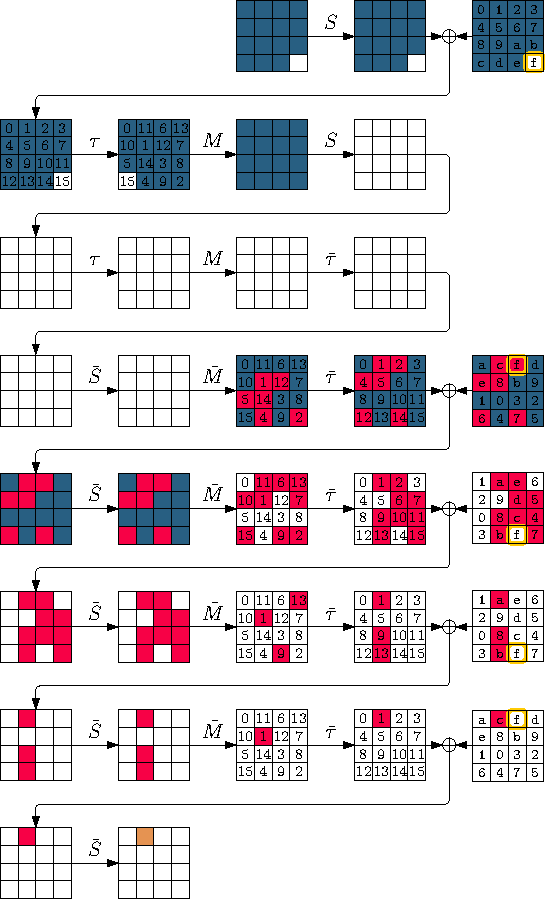
\includegraphics[width=0.52\textwidth]{./figures/qarmav2_64_t1_int_7r.pdf}
\end{center}
\end{columns}
\end{frame}

%%%%%%%%%%%%%%%%%%%%%%%%%%%%%%%%%%%%%%%%%%%%%%%%%%%%%%%%%%%%%%%%%%%%%%%%%%%%%%%
\begin{frame}{ZC Distinguishers for Ciphers Following the \texttt{TWEAKEY} Framework}
\colorlet{char}{tugred} % masks in STK construction
\begin{figure}
  \centering
  \scalebox{0.85}{
  \begin{tikzpicture}[inner sep=1pt,charfont/.style={char,font=\scriptsize}]
    \draw (-1.5,0) node (P)   {$P$}
        ++(0,1.75) node (TK1) {$\TK{1}$}
        ++(0,.5)   node (TK2) {$\TK{2}$}
         +(0,.5)   node       {$\vdots$}
        ++(0,.75)  node (TKz) {$\TK{z}$}
          (9.5,0)  node (C)   {$C$};
    \draw (P.east)   coordinate (Sprev);
    \foreach \t in {1,2,z} {
      \draw (TK\t.east) coordinate (tprev\t); % node[above right,charfont] {$\Lambda_{\t}[i]$};
    }
    % main rounds
    \foreach \rnd/\rndname in {0/0,1/1,2/2,3/r-1} {
      \draw (2*\rnd,0) coordinate[xor] (x\rnd)
          %++(0,.5) node[draw,shape=trapezium,font=\tiny] (expand\rnd) {expand}
          ++(0,.75) coordinate[xor,scale=2] (X\rnd)
          ++(-.75,0) node[font=\tiny] (C\rnd) {$C_{\rndname}$}
          (x\rnd) +(1,0) node[box,minimum width=.45cm,minimum height=.45cm] (f\rnd) {$f$};
      \foreach \t/\toff in {1/-.15,2/0,z/.15} {
        \draw (X\rnd|-TK\t) +(\toff,0) coordinate[tee] (t\t\rnd);
        \draw[every node/.style={circle,draw,inner sep=.5pt,minimum size=.4cm,font=\tiny}]
             (t\t\rnd) ++(.85,0) node (h\t\rnd) {$h$}
                        +(.55,0) node (a\t\rnd) {$\alpha_{\t}$};
        \draw[->] (tprev\t) -- (h\t\rnd);
        \draw (h\t\rnd) -- (a\t\rnd);
        \draw (a\t\rnd.east) coordinate (tprev\t);
        \draw[->,rounded corners=1pt] (t\t\rnd) -- (X\rnd.north-|t\t\rnd) -- (X\rnd);
      }
      \draw[->] (C\rnd) -- (X\rnd);
      \draw[->] (Sprev) -- node[above,charfont] {$\Gamma_{\rndname}$} (x\rnd);
      %\draw[->] (X\rnd) -- (expand\rnd);
      %\draw[->] (expand\rnd) -- (x\rnd);
      \draw[->] (X\rnd) -- (x\rnd);
      \draw[->] (x\rnd) -- (f\rnd);
      \coordinate (Sprev) at (f\rnd.east);
    }
    % last whitening layer
    \draw (2*4+.5,0) coordinate[xor] (x4)
        %++(0,.5) node[draw,shape=trapezium,font=\tiny] (expand4) {expand}
        ++(0,.75) coordinate[xor,scale=2] (X4)
        ++(-.75,0) node[font=\tiny] (C4) {$C_R$};
    \foreach \t/\toff in {1/-.15,2/0,z/.15} {
      \draw (X4|-TK\t) +(\toff,0) coordinate (t\t4);
      \draw[->,rounded corners=1pt] (a\t3.east) -- (t\t4) -- (X4.north-|t\t4) -- (X4);
    }
    \draw[->] (C4) -- (X4);
    \draw[->] (Sprev) -- node[above,charfont] {$\Gamma_R$} (x4);
    %\draw[->] (X4) -- (expand4);
    %\draw[->] (expand4) -- (x4);
    \draw[->] (X4) -- (x4);
    \draw[->] (Sprev) -- (C);
    %
    \draw[above right,charfont]
      (X0.east)+(0,.1) node {$\Gamma_0[i]$}
      (X1.east)+(0,.1) node {$\Gamma_1[h^{-1}(i)]$}
      (X2.east)+(0,.1) node {$\Gamma_2[h^{-2}(i)]$}
      (X3.east)+(0,.1) node {$\Gamma_{r-1}[h^{-r+1}(i)]$}
      (X4.east)+(0,.1) node {$\Gamma_{r}[h^{-r}(i)]$};
    %
    \foreach \etcnode/\etcsize in {f2/.5cm,a12/.42cm,a22/.42cm,az2/.42cm,h12/.42cm,h22/.42cm,hz2/.42cm} {
      \draw (\etcnode.west) ++(-.01,0) node[right,fill=white,minimum width=\etcsize,minimum height=\etcsize] (tmp) {};
      \draw[dotted, thick] (tmp.west) -- (tmp.east);
    }
  \end{tikzpicture}}
\end{figure}
\begin{block}{Ankele et al. \cite{tosc_AnkeleDGLGY2019}}
  \scriptsize
  Let $E_{K}(T, P): \mathbb{F}_{2}^{t\times n}\rightarrow \mathbb{F}_{2}^{n}$ be a TBC following the STK construction.
  Suppose that the tweakey schedule of $E_{K}$ has $z$ parallel paths and applies a permutation $h$ on the tweakey cells in each path.
  Let $(\Gamma_{0}, \Gamma_{r})$ be a pair of linear masks for $r$ rounds of $E_{K}$, and $\Gamma_{1}, \dots, \Gamma_{r - 1}$ represents a possible sequence for the intermediate linear masks.
  If there is a cell position $i$ such that any possible sequence $\Gamma_{0}[i], \Gamma_{1}[h^{-1}(i)], \Gamma_{2}[h^{-2}(i)], \dots \Gamma_{r}[h^{-r}(i)]$ has at most $z$ linearly active cells, 
  then $(\Gamma_{0}, \Gamma_{r})$ yields a ZC linear hull for $r$ rounds of $E$.
\end{block}
\end{frame}

%%%%%%%%%%%%%%%%%%%%%%%%%%%%%%%%%%%%%%%%%%%%%%%%%%%%%%%%%%%%%%%%%%%%%%%%%%%%%%%
\begin{frame}{Example: ZC Distinguisher for Tweakable Block Ciphers}
\vspace{-1.1cm}
\begin{columns}
\column{0.5\textwidth}
\begin{center}
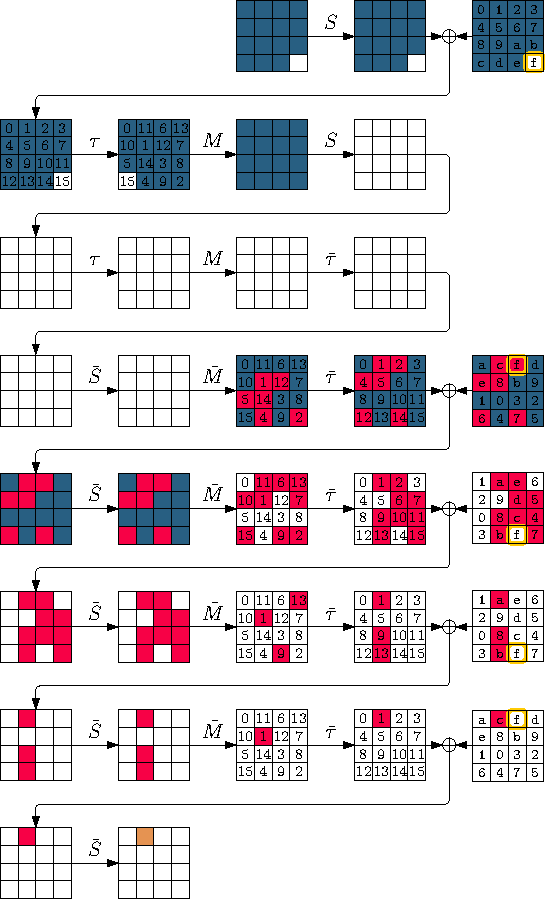
\includegraphics[width=0.5\textwidth]{./figures/qarmav2_64_t1_int_7r.pdf}
\end{center}
\column{0.5\textwidth}
\begin{center}
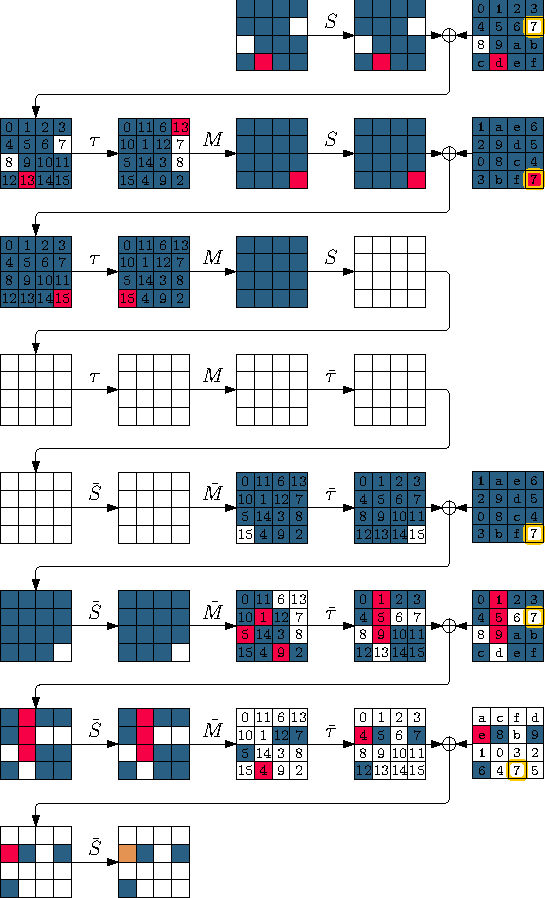
\includegraphics[width=0.5\textwidth]{./figures/qarmav2_64_t1_int_7r_1.pdf}
\end{center}
\end{columns}
\begin{center}
{\scriptsize \scalebox{0.7}{\legendwrap{\Fill[nonzerofixed]{0,0}}}: Fixed nonzero, \scalebox{0.7}{\legendwrap{\Fill[nonzeroany]{0,0}}}: Any nonzero, \scalebox{0.7}{\legendwrap{\Fill[unknown]{0,0}}}: Unknown}
\end{center}
\end{frame}

%%%%%%%%%%%%%%%%%%%%%%%%%%%%%%%%%%%%%%%%%%%%%%%%%%%%%%%%%%%%%%%%%%%%%%%%%%%%%%%
\begin{frame}{CP Model to Search for ZC-based Integral Distinguishers \cite{eurocrypt_HadipourSE23}}
  \begin{columns}
  \column[c]{0.40\textwidth}
  \begin{itemize}
  \item[\faCheckCircleO] \tikzmark{left}$\csp\Up(\Gamma\Up)$
  \item[\faCheckCircleO] $\csp\Low(\Gamma\Low)$
  \item[\faCheckCircleO] \textcolor{tugred}{$\csp_{\texttt{M}}(\Gamma\Up, \Gamma\Low)$}\tikzmark{right}
  \item[\faCheckCircle] $\csp\Dist = \csp\Up \wedge \csp\Low \wedge \csp_{\texttt{M}}$
  \end{itemize}
  \column[c]{0.60\textwidth}
  \begin{figure}
  \centering
  \begin{tikzpicture}[xscale=1.2,yscale=1, charfont/.style={char,font=\scriptsize}]
  \pgfmathsetmacro{\dx}{0.45}
  \pgfmathsetmacro{\dy}{0.35}
  \pgfmathsetmacro{\lxe}{2.5}
  \pgfmathsetmacro{\lye}{1.2}
  \coordinate (tleu) at (0,0);
  
  \draw[rounded corners=0.1cm] (tleu) rectangle ++(2*\lxe,-\lye) coordinate (breu);
  \node at ($(tleu)!0.5!(breu) + (0, 1.2*\dy)$) {\textcolor{tugblue}{$E\Up$}};
  \draw[rounded corners=0.1cm] (breu) ++(-2*\lxe, -\dy) coordinate (tlel) rectangle ++(2*\lxe,-\lye) coordinate (brel);
  \node at ($(tlel)!0.5!(brel) + (0, 1.2*\dy)$) {\textcolor{tugblue}{$E\Low$}};

  \draw[|<-|, postaction={decorate}, thin, dashed] ($(tlel) + (0, -\lye - 0.2)$) -- node[below] {$r\Dist$} ($(brel) + (0, -0.2)$);
  
  \fill[fill=tuggray, opacity=0.6] ($(tleu) + (0, -\lye/2 + 0.05)$) -- ($(tleu) + (0, -\lye/2 - 0.05)$) -- ($(breu) + (0, 0.1)$) -- ($(breu) + (0, \lye - 0.1)$) -- cycle;
  \fill[fill=tugred, opacity=0.6] ($(tlel) + (0, -0.1)$) -- ($(tlel) + (0, -\lye + 0.1)$) -- ($(brel) + (0, \lye/2 - 0.05)$) -- ($(brel) + (0, \lye/2 + 0.05)$) -- cycle;
  
  \coordinate (deltaup) at ($(tleu) + (-\dx*1.3, -\lye/2)$);
  \coordinate (deltalowl) at ($(brel) + (+\dx*1.3, +\lye/2)$);
  
  \draw[->] (deltaup) -- node[above] {$\Gamma\Up$} (deltaup-|tleu);
  \draw[->] (deltalowl) -- node[above] {$\Gamma\Low$} (deltalowl-|brel);
  
  \node[rotate=90] at ($(tleu) + (\lxe/8,-\lye/2)$) (u1) {$\axu_{0}$};
  \node[rotate=90] at ($(tleu) + (\lxe*3/8,-\lye/2)$) (u2) {$\axu_{1}$};
  \node[rotate=00] at ($(tleu) + (\lxe*5/8,-\lye/2)$) (u3) {$\cdots$};
  \node[rotate=90] at ($(breu) + (-\lxe/8,+\lye/2)$) (u4) {$\axu_{r\Dist}$};
  
  \node[rotate=90] at ($(tlel) + (\lxe/8,-\lye/2)$) (l1) {$\axl_{0}$};
  \node[rotate=90] at ($(tlel) + (\lxe*3/8,-\lye/2)$) (l2) {$\axl_{1}$};
  \node[rotate=00] at ($(tlel) + (\lxe*5/8,-\lye/2)$) (l3) {$\cdots$};
  \node[rotate=90] at ($(brel) + (-\lxe/8,+\lye/2)$) (l4) {$\axl_{r\Dist}$};
  
  \draw ($0.5*(u1) + 0.5*(l1)$) node[tugred] {\faBolt};
  \draw ($0.5*(u2) + 0.5*(l2)$) node[tugred] {\faBolt};
  \draw ($0.5*(u3) + 0.5*(l3)$) node[tugred] {\faBolt};
  \draw ($0.5*(u4) + 0.5*(l4)$) node[tugred] {\faBolt};

  \end{tikzpicture}
  \end{figure}
  \end{columns}
  \end{frame}

%%%%%%%%%%%%%%%%%%%%%%%%%%%%%%%%%%%%%%%%%%%%%%%%%%%%%%%%%%%%%%%%%%%%%%%%%%%%%%%
%%%%%%%%%%%%%%%%%%%%%%%%%%%%%%%%%%%%%%%%%%%%%%%%%%%%%%%%%%%%%%%%%%%%%%%%%%%%%%%
\section{Properties of MixColumns of \texttt{QARMAv2}}
\sectionheader[\huge\color{tug}\faLightbulbO]{Properties of MixColumns of \texttt{QARMAv2}}

\begin{frame}{Properties of MixColumns of \texttt{QARMAv2}}
\sparen
\begin{itemize}
  \item MixColumns of \texttt{QARMAv2} is defined as follows:
\begin{equation*}
  \label{eq:bypass_mixcolumns_property}
  \begin{pmatrix}
    Y_0\\
    Y_1\\
    Y_2\\
    Y_3
  \end{pmatrix} = 
  \begin{pmatrix}
    0 & \rho & \rho^2 & \rho^3\\
    \rho^3 & 0 & \rho & \rho^2\\
    \rho^2 & \rho^3 & 0 & \rho\\
    \rho & \rho^2 & \rho^3 & 0
  \end{pmatrix} \times
  \begin{pmatrix}
    X_0\\
    X_1\\
    X_2\\
    X_3
  \end{pmatrix} = 
  \begin{pmatrix}
    \rho X_1 + \rho^2 X_2 + \rho^3 X_3\\
    \rho^3 X_0 + \rho X_2 + \rho^2 X_3\\
    \rho^2 X_0 + \rho^3 X_1 + \rho X_3\\
    \rho X_0 + \rho^2 X_1 + \rho^3 X_2
  \end{pmatrix}.
\end{equation*}
\item $\rho$: rotation to the left by 1 bit, and $\rho^{4} = 1$.
\item If $X_{i}$ and $X_{j}$ have the zero-sum property simultaneously, then a linear combination of $Y_{i}$ and $Y_{j}$ also has the zero-sum property:
\[\bigoplus_{c\in \mathbb{C}} \left((\rho^{(i - j)\!\!\!\mod 4} X_i(c)) \oplus X_{j}(c)\right) = \bigoplus_{c \in \mathbb{C}} \left((\rho^{(i - j)\!\!\!\mod 4} Y_i(c)) \oplus Y_j(c)\right).\]
\end{itemize}
\end{frame}
%%%%%%%%%%%%%%%%%%%%%%%%%%%%%%%%%%%%%%%%%%%%%%%%%%%%%%%%%%%%%%%%%%%%%%%%%%%%%%%
%%%%%%%%%%%%%%%%%%%%%%%%%%%%%%%%%%%%%%%%%%%%%%%%%%%%%%%%%%%%%%%%%%%%%%%%%%%%%%%
\section{Our Method to Search For Distinguisher}
\sectionheader[\huge\color{tug}\faLightbulbO]{Our Method to Search for Distinguishers}

%%%%%%%%%%%%%%%%%%%%%%%%%%%%%%%%%%%%%%%%%%%%%%%%%%%%%%%%%%%%%%%%%%%%%%%%%%%%%%%
\begin{frame}{Our Method to Search for ZC-based Integral Distinguishers}
\begin{columns}
\column[c]{0.40\textwidth}
\begin{itemize}
\item[\faCheckCircleO] \tikzmark{left}$\csp\Up(\Gamma\Up)$
\item[\faCheckCircleO] $\csp1\Low(\Gamma1\Low)$
\item[\faCheckCircleO] $\csp2\Low(\Gamma2\Low)$
\item[\faCheckCircleO] \textcolor{tugred}{$\csp_{\texttt{M}}(\Gamma\Up, \Gamma1\Low, \Gamma2\Low)$}\tikzmark{right}
\item[\faCheckCircle] $\csp\Up \wedge \csp1\Low \wedge \csp2\Low \wedge \csp_{\texttt{M}}$
\end{itemize}
\column[c]{0.60\textwidth}
\begin{figure}
\centering
\begin{tikzpicture}[xscale=1.2,yscale=1, charfont/.style={char,font=\scriptsize}]
\pgfmathsetmacro{\dx}{0.45}
\pgfmathsetmacro{\dy}{0.35}
\pgfmathsetmacro{\lxe}{2.5}
\pgfmathsetmacro{\lye}{1.2}
\coordinate (tleu) at (0,0);

\draw[rounded corners=0.1cm] (tleu) rectangle ++(2*\lxe,-\lye) coordinate (breu);
\node at ($(tleu)!0.5!(breu) + (0, 1.2*\dy)$) {\textcolor{tugblue}{$E\Up$}};
\draw[rounded corners=0.1cm] (breu) ++(-2*\lxe, -\dy) coordinate (tlel) rectangle ++(2*\lxe,-\lye) coordinate (brel);
\node at ($(tlel)!0.5!(brel) + (0, 1.2*\dy)$) {\textcolor{tugblue}{$E\Low$}};
\draw[rounded corners=0.1cm] (tleu)++(0, \lye+\dy) coordinate (tlell) rectangle ++(2*\lxe,-\lye) coordinate (brell);
\node at ($(tlell)!0.5!(brell) + (0, 1.2*\dy)$) {\textcolor{tugblue}{$E\Low$}};

\draw[|<-|, postaction={decorate}, thin, dashed] ($(tlell) + (0, 0.2)$) -- node[above] {$r\Dist$} ($(brell) + (0,\lye + 0.2)$);
\draw[|<-|, postaction={decorate}, thin, dashed] ($(tlel) + (0, -\lye - 0.2)$) -- node[below] {$r\Dist$} ($(brel) + (0, -0.2)$);

\fill[fill=tuggray, opacity=0.6] ($(tleu) + (0, -\lye/2 + 0.05)$) -- ($(tleu) + (0, -\lye/2 - 0.05)$) -- ($(breu) + (0, 0.1)$) -- ($(breu) + (0, \lye - 0.1)$) -- cycle;
\fill[fill=tugred, opacity=0.6] ($(tlel) + (0, -0.1)$) -- ($(tlel) + (0, -\lye + 0.1)$) -- ($(brel) + (0, \lye/2 - 0.05)$) -- ($(brel) + (0, \lye/2 + 0.05)$) -- cycle;
\fill[fill=tugblue, opacity=0.6] ($(tlell) + (0, -0.1)$) -- ($(tlell) + (0, -\lye + 0.1)$) -- ($(brell) + (0, \lye/2 - 0.05)$) -- ($(brell) + (0, \lye/2 + 0.05)$) -- cycle;

\coordinate (deltaup) at ($(tleu) + (-\dx*1.3, -\lye/2)$);
\coordinate (deltalowl) at ($(brel) + (+\dx*1.3, +\lye/2)$);
\coordinate (deltalowll) at ($(brell) + (+\dx*1.3, +\lye/2)$);

\draw[->] (deltaup) -- node[above] {$\Gamma\Up$} (deltaup-|tleu);
\draw[->] (deltalowl) -- node[above] {$\Gamma1\Low$} (deltalowl-|brel);
\draw[->] (deltalowll) -- node[above] {$\Gamma2\Low$} (deltalowll-|brel);

\node[rotate=90] at ($(tleu) + (\lxe/8,-\lye/2)$) (u1) {$\axu_{0}$};
\node[rotate=90] at ($(tleu) + (\lxe*3/8,-\lye/2)$) (u2) {$\axu_{1}$};
\node[rotate=00] at ($(tleu) + (\lxe*5/8,-\lye/2)$) (u3) {$\cdots$};
\node[rotate=90] at ($(breu) + (-\lxe/8,+\lye/2)$) (u4) {$\axu_{r\Dist}$};

\node[rotate=90] at ($(tlel) + (\lxe/8,-\lye/2)$) (l1) {$\axl1_{0}$};
\node[rotate=90] at ($(tlel) + (\lxe*3/8,-\lye/2)$) (l2) {$\axl1_{1}$};
\node[rotate=00] at ($(tlel) + (\lxe*5/8,-\lye/2)$) (l3) {$\cdots$};
\node[rotate=90] at ($(brel) + (-\lxe/8,+\lye/2)$) (l4) {$\axl1_{r\Dist}$};

\node[rotate=90] at ($(tlell) + (\lxe/8,-\lye/2)$) (ll1) {$\axl2_{0}$};
\node[rotate=90] at ($(tlell) + (\lxe*3/8,-\lye/2)$) (ll2) {$\axl2_{1}$};
\node[rotate=00] at ($(tlell) + (\lxe*5/8,-\lye/2)$) (ll3) {$\cdots$};
\node[rotate=90] at ($(brell) + (-\lxe/8,+\lye/2)$) (ll4) {$\axl2_{r\Dist}$};

\draw ($0.5*(u1) + 0.5*(l1)$) node[tugred] {\faBolt};
\draw ($0.5*(u2) + 0.5*(l2)$) node[tugred] {\faBolt};
\draw ($0.5*(u3) + 0.5*(l3)$) node[tugred] {\faBolt};
\draw ($0.5*(u4) + 0.5*(l4)$) node[tugred] {\faBolt};

\draw ($0.5*(u1) + 0.5*(ll1)$) node[tugred] {\faBolt};
\draw ($0.5*(u2) + 0.5*(ll2)$) node[tugred] {\faBolt};
\draw ($0.5*(u3) + 0.5*(ll3)$) node[tugred] {\faBolt};
\draw ($0.5*(u4) + 0.5*(ll4)$) node[tugred] {\faBolt};
\end{tikzpicture}
\end{figure}
\end{columns}
\end{frame}

%%%%%%%%%%%%%%%%%%%%%%%%%%%%%%%%%%%%%%%%%%%%%%%%%%%%%%%%%%%%%%%%%%%%%%%%%%%%%%%
\begin{frame}{Example of Our Method to Search for Distinguishers}
\vspace{-1.1cm}
\begin{columns}
\column{0.5\textwidth}
\begin{center}
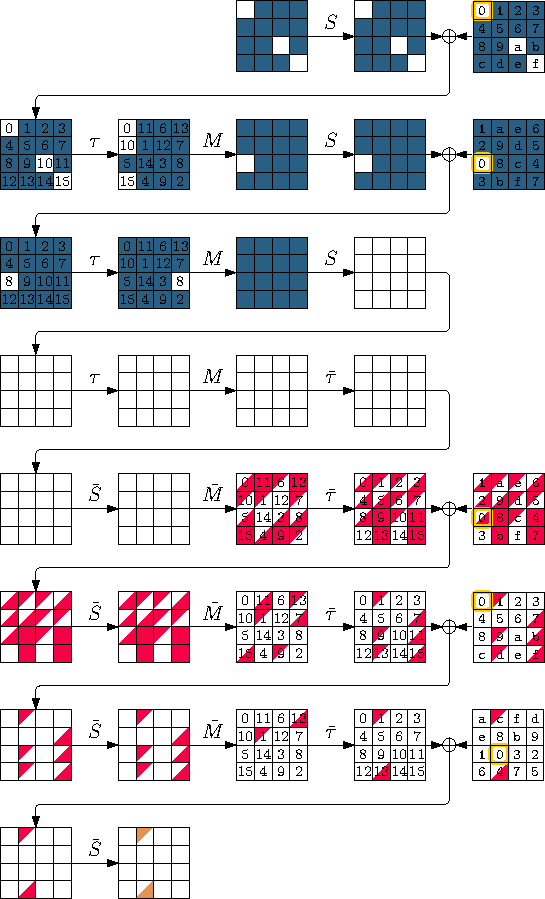
\includegraphics[width=0.5\textwidth]{./figures/example1.pdf}
\end{center}
\column{0.5\textwidth}
\begin{center}
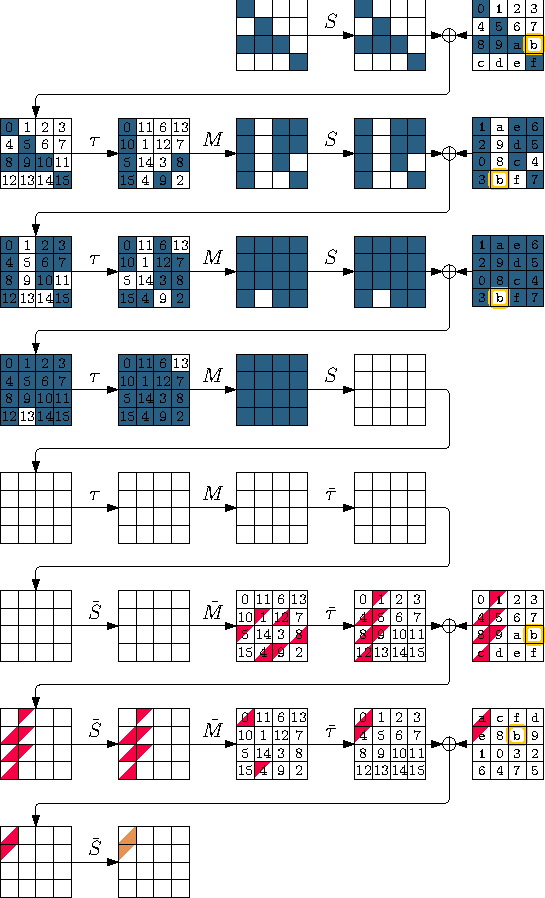
\includegraphics[width=0.5\textwidth]{./figures/example2.pdf}
\end{center}
\end{columns}
\begin{center}
{\scriptsize \scalebox{0.7}{\legendwrap{\Fill[nonzerofixed]{0,0}}}: Fixed nonzero, \scalebox{0.7}{\legendwrap{\Fill[nonzeroany]{0,0}}}: Any nonzero, \scalebox{0.7}{\legendwrap{\Fill[unknown]{0,0}}}: Unknown}
\end{center}
\end{frame}

%%%%%%%%%%%%%%%%%%%%%%%%%%%%%%%%%%%%%%%%%%%%%%%%%%%%%%%%%%%%%%%%%%%%%%%%%%%%%%%
%%%%%%%%%%%%%%%%%%%%%%%%%%%%%%%%%%%%%%%%%%%%%%%%%%%%%%%%%%%%%%%%%%%%%%%%%%%%%%%
\section{Key Recovery Attack on \texttt{QARMAv2}} 
\sectionheader[\huge\color{tug}\faKey]{Key Recovery Attack on \texttt{QARMAv2}}

\begin{frame}{Naive Approach v.s. MitM \cite{sacryptSasaki012}}
\vspace{-0.5cm}
\begin{columns}
\column[c]{.6\textwidth}
\begin{itemize}
\item[\faCab] Naive approach:
\begin{itemize}
	\item[\faCheckCircleO] $\bm{x} = F(\bm{k}_{1}, \bm{k}_{2}, \bm{c})$ 
	\item[\faCheckCircleO] $T = N \cdot 2^{|\bm{k}_{1} \cup \bm{k}_{2}|}$
\end{itemize}
\item<2->[\faFighterJet] MitM:
\begin{itemize}
	\item <2->[\faCheckCircle] $\bm{x} = g(\bm{k}_{1}, \bm{c}),\, \bm{y} = h(\bm{k}_{2}, \bm{c})$
	\item <2->[\faCheckCircle] $T = N \cdot 2^{|\bm{k}_{1}|} + N \cdot 2^{|\bm{k}_{2}|}$
\end{itemize}
\end{itemize}
\column[c]{0.4\textwidth}
\centering
\null
\vspace{0.5cm}
\begin{figure}
\centering
\begin{tikzpicture}[yscale=1, xscale=1, thick, >=latex,
every node/.style={inner sep=6pt},
next/.append style={rounded corners=3pt},
primi/.append style={fill=tugred!50, draw=black, rounded corners=2pt, minimum size=30pt},
caption/.style={gray, below=1.75cm, align=center}]
\node[primi, key north, fill=tugblue] (E1) {\textcolor{white}{\texttt{Path 1}}};
\draw[next]  (E1) ++(0,1) node[right]{$\bm{k}_{1}$\,\faKey} -- (E1);
\draw[next]  (E1) ++(1.5,0) node[right]{$\bm{c}$} -- (E1);
\node[primi, below=0.7cm of E1, key north, fill=tugred] (E2) {\textcolor{white}{\texttt{Path 2}}};
\draw[next]  (E2) ++(0,1) node[right]{$\bm{k}_{2}$\,\faKey} -- (E2);
\draw[<-] (E2) -- ++(1.5, 0) node[right]{$\bm{c}$};
\node[xor, minimum size=0.4cm] at ($(E1)!0.5!(E2) + (-1.5, 0)$) (myxor) {};
\draw[->, rounded corners] (E1) --node[above]{$\bm{x}$} (E1-|myxor) -- (myxor.north);
\draw[->, rounded corners] (E2) --node[below]{$\bm{y}$} (E2-|myxor) -- (myxor.south);
\node[left=1cm of myxor] (Z) {$\bm{z}$};
\draw[->] (myxor) -- (Z);
\end{tikzpicture}
\end{figure}
\[\visible<1->{\sum_{c\in \bm{c}} \bm{z} = 0} \visible<2->{\iff \sum_{c \in \bm{c}} \bm{x} = \sum_{c \in \bm{c}} \bm{y}}\]
\end{columns}
\end{frame}

%%%%%%%%%%%%%%%%%%%%%%%%%%%%%%%%%%%%%%%%%%%%%%%%%%%%%%%%%%%%%%%%%%%%%%%%%%%%%%%
\begin{frame}{Naive Approach v.s. Partial-Sum Technique \cite{fseFergusonKLSSWW00}}
\vspace{-0.5cm}
\begin{columns}
\column[c]{.62\textwidth}
\begin{itemize}
\small
\item[\faCab] Naive approach:
\begin{itemize}
  \small
	\item[\faCheckCircleO] $\bm{x} = F(\bm{k}, \bm{c})$ 
	\item[\faCheckCircleO] $T = N \cdot 2^{|\bm{k}|}$
\end{itemize}
\item<2->[\faFighterJet] Partial-sum technique:
\begin{itemize}
  \small
	\item<2->[\faCheckCircle] $\!\bm{x}_{1}\!=\!f_{1}(\bm{k}_{1}, \bm{x}_{0}),\!\bm{x}_{2}\!=\!f_{2}(\bm{k}_{2},\!\bm{x}_{1})\!,\cdots\!,\!\bm{x}\!=\!f_{n}(\bm{k}_{n}, \bm{x}_{n-1})$	
	\item<2->[\faCheckCircle] $\!\bm{x}_{0} = \bm{c}, N_{0} = N, N_{i} < N$
	\item<2->[\faCheckCircle] $\!T = \sum_{i = 1}^{n} \frac{N_{i - 1}}{n}\cdot 2^{|\bm{k}_{1}| + \cdots + |\bm{k}_{i}|} < \sum_{i = 1}^{n} \frac{N}{n} \cdot 2^{|\bm{k}|}$
	\item<2->[\faCheckCircle] $T < N\cdot 2^{|\bm{k}|}$ 
\end{itemize}
\end{itemize}
\column[c]{0.38\textwidth}
\centering
\null
\vspace{0.5cm}
\begin{figure}
\centering
\begin{subfigure}{0.49\textwidth}
\centering
\begin{tikzpicture}[xscale=1,yscale=1, charfont/.style={font=\scriptsize}]
\pgfmathsetmacro{\dx}{0.7}
\pgfmathsetmacro{\hdx}{\dx/2}
\pgfmathsetmacro{\dy}{0.5}
\pgfmathsetmacro{\hdy}{\dy/2}
\pgfmathsetmacro{\lxe}{2.7}
\pgfmathsetmacro{\lye}{1.2}
\coordinate (tleu) at (0,0);
\draw[rounded corners=0.1cm] (tleu) rectangle ++(\lxe,-\lye) coordinate (breu);
\coordinate (meu) at ($(tleu)!0.5!(breu)$);
\node at ($(tleu)!0.5!(breu) + (0, 0.7*\dy)$) {\textcolor{tugred}{$F$}};
\fill[fill=tuggray, opacity=0.6] ($(tleu) + (0, -\lye/2 + 0.05)$) -- ($(tleu) + (0, -\lye/2 - 0.05)$) -- ($(breu) + (0, 0.1)$) -- ($(breu) + (0, \lye - 0.1)$) -- cycle;
\node (x) at ($(tleu|-meu)+(-\dx,0)$) {$\bm{x}$};
\node (c) at ($(breu|-meu)+(\dx,0)$) {$\bm{c}$};
\node (k) at ($(tleu-|meu)+(0,1.5*\dy)$) {$\bm{k}$};
\draw[->] (c) -- ++(-\dx, 0);
\draw[<-] (x) -- ++(\dx, 0);
\draw[->] (k) -- ++(0, -1.5*\dy);
\end{tikzpicture}
\end{subfigure}
\vskip 0.5cm

\visible<2>{
\begin{subfigure}{0.49\textwidth}
\centering
\begin{tikzpicture}[xscale=1,yscale=1, charfont/.style={font=\scriptsize}]
\pgfmathsetmacro{\dx}{0.7}
\pgfmathsetmacro{\hdx}{\dx/2}
\pgfmathsetmacro{\dy}{0.5}
\pgfmathsetmacro{\hdy}{\dy/2}
\pgfmathsetmacro{\lxe}{2.7}
\pgfmathsetmacro{\lye}{1.2}
\coordinate (tleu) at (0,0);
\draw[rounded corners=0.1cm] (tleu) rectangle ++(\lxe,-\lye) coordinate (breu);
\coordinate (meu) at ($(tleu)!0.5!(breu)$);
\node at ($(tleu)!0.5!(breu) + (0, 0.7*\dy)$) {\textcolor{tugred}{$F$}};
\fill[fill=tuggray, opacity=0.6] ($(tleu) + (0, -\lye/2 + 0.05)$) -- ($(tleu) + (0, -\lye/2 - 0.05)$) -- ($(breu) + (0, 0.1)$) -- ($(breu) + (0, \lye - 0.1)$) -- cycle;
\node (x) at ($(tleu|-meu)+(-\dx,0)$) {$\bm{x}$};
\node (c) at ($(breu|-meu)+(\dx,0)$) {$\bm{c}$};
\node (k) at ($(tleu-|meu)+(0,1.5*\dy)$) {};
\draw[->] (c) -- ++(-\dx, 0);
\draw[<-] (x) -- ++(\dx, 0);

\node[] (x1) at ($(breu) + (-\lxe/8,+\lye/2)$) {$\bm{x}_{1}$};
\node[] (x2) at ($(breu) + (-\lxe*3/8,+\lye/2)$) {$\bm{x}_{2}$};
\node[rotate=00] (td) at ($(breu) + (-\lxe*5/9,+\lye/2)$) {$\cdots$};
\node[] (xn) at ($(tleu) + (\lxe/6,-\lye/2)$) {$\bm{x}_{n - 1}$};
\node (k1) at (x1|-k) {$\bm{k}_{1}$};
\node (k2) at (x2|-k) {$\bm{k}_{2}$};
\node (ttd) at (td|-k) {$\cdots$};
\node (kn) at (xn|-k) {$\bm{k}_{n}$};
\draw[->] (k1) -- ++(0, -1.5*\dy);
\draw[->] (k2) -- ++(0, -1.5*\dy);
\draw[->] (kn) -- ++(0, -1.5*\dy);
\end{tikzpicture}
\end{subfigure}}
\end{figure}
\end{columns}
\end{frame}

%%%%%%%%%%%%%%%%%%%%%%%%%%%%%%%%%%%%%%%%%%%%%%%%%%%%%%%%%%%%%%%%%%%%%%%%%%%%%%%
%%%%%%%%%%%%%%%%%%%%%%%%%%%%%%%%%%%%%%%%%%%%%%%%%%%%%%%%%%%%%%%%%%%%%%%%
\begin{frame}{Example: Partial-Sum Technique \cite{fseFergusonKLSSWW00}}
\begin{columns}
\sparen
\column[c]{0.50\textwidth}
\centering
\resizebox{\textwidth}{!}{%
\begin{tikzpicture}[>=latex,xscale=1.35,remember picture,
                    stateopts/.style={scale=.25},
                    sbox/.style={draw,rounded corners=3pt, scale=.6}]
  \pgfmathsetmacro{\statesep}{1.5}

  \draw[every node/.style={state}] %, rounded corners=2pt]
  (-1, 0) node (SI) {\State{\Cell{ss00}{\tiny \texttt{0}} \Cell{ss10}{\tiny \texttt{1}} \Cell{ss20}{\tiny \texttt{2}} \Cell{ss30}{\tiny \texttt{3}}
  \Cell{ss01}{\tiny \texttt{4}} \Cell{ss11}{\tiny \texttt{5}} \Cell{ss21}{\tiny \texttt{6}} \Cell{ss31}{\tiny \texttt{7}}
  \Cell{ss02}{\tiny \texttt{8}} \Cell{ss12}{\tiny \texttt{9}} \Cell{ss22}{\tiny \texttt{10}}\Cell{ss32}{\tiny \texttt{11}}
  \Cell{ss03}{\tiny \texttt{12}} \Cell{ss13}{\tiny \texttt{13}} \Cell{ss23}{\tiny \texttt{14}} \Cell{ss33}{\tiny \texttt{15}}
  \iAct{ss00}\iAct{ss11}\iAct{ss22}\iAct{ss33}}}
  ++(0.9,-.9) node (SKI) {\State{\Cell{ss00}{\tiny \texttt{0}} \Cell{ss10}{\tiny \texttt{1}} \Cell{ss20}{\tiny \texttt{2}} \Cell{ss30}{\tiny \texttt{3}}
  \Cell{ss01}{\tiny \texttt{4}} \Cell{ss11}{\tiny \texttt{5}} \Cell{ss21}{\tiny \texttt{6}} \Cell{ss31}{\tiny \texttt{7}}
  \Cell{ss02}{\tiny \texttt{8}} \Cell{ss12}{\tiny \texttt{9}} \Cell{ss22}{\tiny \texttt{10}}\Cell{ss32}{\tiny \texttt{11}}
  \Cell{ss03}{\tiny \texttt{12}} \Cell{ss13}{\tiny \texttt{13}} \Cell{ss23}{\tiny \texttt{14}} \Cell{ss33}{\tiny \texttt{15}}
  }} ++(.65,-.4) node {\footnotesize $K_{0}$};
  \draw (SI) ++(0.9,0) coordinate[xor] (xori);
  \draw[->] (SI.east) -- (xori);
  \draw[->] (SKI) -- (xori);  
  % States
  \draw[every node/.style={state}] %, rounded corners=2pt]        
  ++(\statesep,0) node (S4) {\State{\foreach \b in {0,...,15} {\iBal{s\b}}}}
  ++(\statesep,0) +(0,-.9) node (SK5) {\State{\iKey{s0}{4} }}
  ++(0.65*\statesep,0) node (S5) {\State{\iPartial{s0}{4} }}
  ++(\statesep,0) +(0,-.9) node (SK6) {\State{\foreach \b/\s in {0/1,7/3,10/2,13/1} {\iKey{s\b}{\s}} }}
  ++(\statesep*.75,0) node (S6) {\State{\foreach \b/\s in {0/1,7/3,10/2,13/1} {\iStep{s\b}{\s}} }};
  \draw[->] (xori) -- node[above]{\small 4 rounds} (S4.west);
  \draw (S4) ++(0,-.8) node {\footnotesize $C_4$};
  \draw (S5) ++(0,-.8) node {\footnotesize $C_5$};
  \draw (S6) ++(0,-.8) node {\footnotesize $C_6$};
  \draw (SK5) ++(.65,-.4) node {\footnotesize $\bar{K}_5$};
  \draw (SK6) ++(.65,-.4) node {\footnotesize $K_6$};

  % Operations
  % \draw (\statesep/2,0) node[font=\fontsize{5}{5}\selectfont,align=center] {SB\\SR\\MC\\AK};
  \draw ($(S4.east) + (0.2, 0)$) node[font=\fontsize{5}{5}\selectfont,align=center] (Op5) {SB\\SR};
  \draw ($(S5.east) + (0.2, 0)$) node[font=\fontsize{5}{5}\selectfont,align=center] (Op6) {MC\\SB\\SR};


  \foreach \r in {5,6} {
    \draw (SK\r) ++(0,.9) coordinate[xor] (xor\r);
    \draw[->] (xor\r.east) -- (S\r.west);
    \draw[->] (Op\r.east) -- (xor\r.west);
    \draw[->] (SK\r.north) -- (xor\r.south);
  }
\end{tikzpicture}}
\sparen
\sparen
\begin{itemize}
  \scriptsize
  \item Guess $K_{6}[0, 7]$ and derive $\mathcal{S}_{0}\left(C_{6}[0]\oplus K_{6}[0]\right) \oplus \mathcal{S}_{1}\left(C_{6}[7] \oplus K_{6}[7]\right)$
  \sparen
  \item Guess $K_{6}[10]$ and derive $\mathcal{S}_{2}\left(C_{6}[10] \oplus K_{6}[10]\right)$
  \sparen
  \item Guess $K_{6}[13]$ and derive $\mathcal{S}_{3}\left(C_{6}[13] \oplus K_{6}[13]\right)$
  \sparen
  \item Guess $\bar{K}_{5}[0]$ and derive $C_{4}[0]$
  \sparen
  \item Time complexity: $6\times 4\times 2^{48} \approx 2^{52}$ S-box lookups 
\end{itemize}
\column[c]{0.50\textwidth}
\centering
%\begin{tikzpicture}[>=latex,xscale=1.25,yscale=\PScale,remember picture]
\resizebox{\textwidth}{!}{%
\begin{tikzpicture}[xscale=1.25,yscale=\PScale,remember picture,
                    sbox/.style={draw,rounded corners=3pt, scale=.6}]
  \pgfmathsetmacro{\statesep}{1.5}

  \draw (0, -3) node[inner sep=0pt] (S51) {\PartialSumStepInit}
  ++(0, -2.67) node[inner sep=0pt] (S52) {\PartialSumStepTwo}
  ++(0, -2.42) node[inner sep=0pt] (S53) {\PartialSumStepThree}
  ++(0, -1.83) node[inner sep=0pt] (S54) {\PartialSumStepFinal};
  \draw (sbox.south) coordinate (branch1);

  \draw (S51.north) ++(0,.3) node[inner sep=0pt] (X) {\footnotesize $C^0$};
  
  \draw (S51.north west) ++(-.3,0) node[inner sep=0pt, anchor=north east, align=right] (X) {\footnotesize Step 1: $\text{Key}= 2^{16}$ \\ \footnotesize $\text{Data} = 2^{32}$ \\ \footnotesize $\text{Time} = 2^{48}$};
  \draw (S52.north west) ++(-.3,0) node[inner sep=0pt, anchor=north east, align=right] (X) {\footnotesize Step 2: $\text{Key}= 2^{24}$ \\ \footnotesize $\text{Data} = 2^{24}$ \\ \footnotesize $\text{Time} = 2^{48}$};
  \draw (S53.north west) ++(-.3,0) node[inner sep=0pt, anchor=north east, align=right] (X) {\footnotesize Step 3: $\text{Key}= 2^{32}$ \\ \footnotesize $\text{Data} = 2^{16}$ \\ \footnotesize $\text{Time} = 2^{48}$};
  \draw (S54.north west) ++(-.3,0) node[inner sep=0pt, anchor=north east, align=right] (X) {\footnotesize Step 4: $\text{Key}= 2^{40}$ \\ \footnotesize $\text{Data} = 2^{8}$ \\ \footnotesize $\text{Time} = 2^{48}$};

  % \draw (3, -3) node[inner sep=0pt] (S51) {\PartialSumStepInit}
  % ++(0, -2.67) node[inner sep=0pt] (S52) {\PartialSumStepTwo}
  % ++(0, -2.42) node[inner sep=0pt] (S53) {\PartialSumStepThree}
  % ++(0, -1.83) node[inner sep=0pt] (S54) {\PartialSumStepFinal};
  % \draw (sbox.south) coordinate (branch2);

  % \draw (S51.north) ++(0,.3) node[inner sep=0pt] (X) {\footnotesize $C^1$};
  \draw (2,-6) node (dots) {$\dots$};

  \draw (4.5, -3) node[inner sep=0pt] (S51) {\PartialSumStepInit}
  ++(0, -2.67) node[inner sep=0pt] (S52) {\PartialSumStepTwo}
  ++(0, -2.42) node[inner sep=0pt] (S53) {\PartialSumStepThree}
  ++(0, -1.83) node[inner sep=0pt] (S54) {\PartialSumStepFinal};
  \draw (sbox.south) coordinate (branchn);

  \draw (S51.north) ++(0,.3) node[inner sep=0pt] (X) {\footnotesize $C^{2^{32}-1}$};

  \draw (branch1-|dots) ++(0,-.2) coordinate[xor] (xor5);
  \draw (xor5) ++(0,-.5) node[inner sep=0pt] (c5) {\SingleCell{\iBal{s}}};
  \draw (c5.west) ++(-.05,0) node[inner sep=0pt, anchor=east] {\footnotesize is};
  \draw (c5.east) ++(.05,0) node[inner sep=0pt, anchor=west] {\footnotesize ?};
  \draw[->, rounded corners=2pt] (xor5.south) -- (c5.north);

  \draw[->, rounded corners=2pt] (branch1) |- (xor5.west);
  \draw[->, rounded corners=2pt] (branchn) |- (xor5.east);

  \draw (xor5-|dots) ++(1,0) node[inner sep=5pt,fill=white] {$\dots$};

\end{tikzpicture}}
\end{columns}
\end{frame}

%%%%%%%%%%%%%%%%%%%%%%%%%%%%%%%%%%%%%%%%%%%%%%%%%%%%%%%%%%%%%%%%%%%%%%%%%%%%%%%
\begin{frame}{13-Round Integral Attack on \texttt{QARMAv2}-64-128 ($\mathscr{T} = 1$) I}
\vspace{-1cm}
\begin{columns}
\column{0.3\textwidth}
\begin{center}
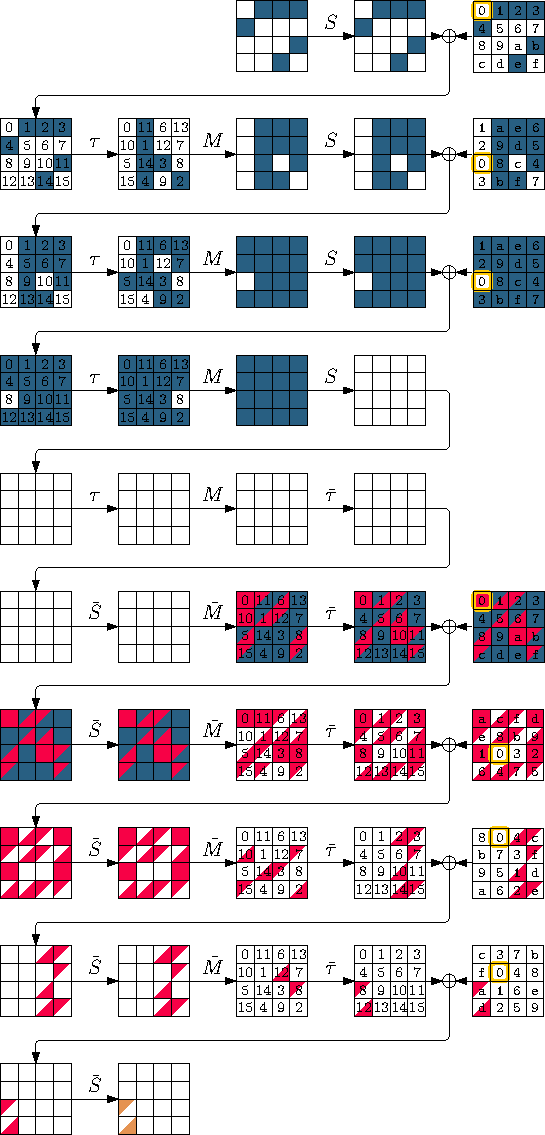
\includegraphics[width=0.67\textwidth]{./figures/qarmav2_64_t1_9r_v0.pdf}
\end{center}
\column{0.7\textwidth}
\begin{center}
  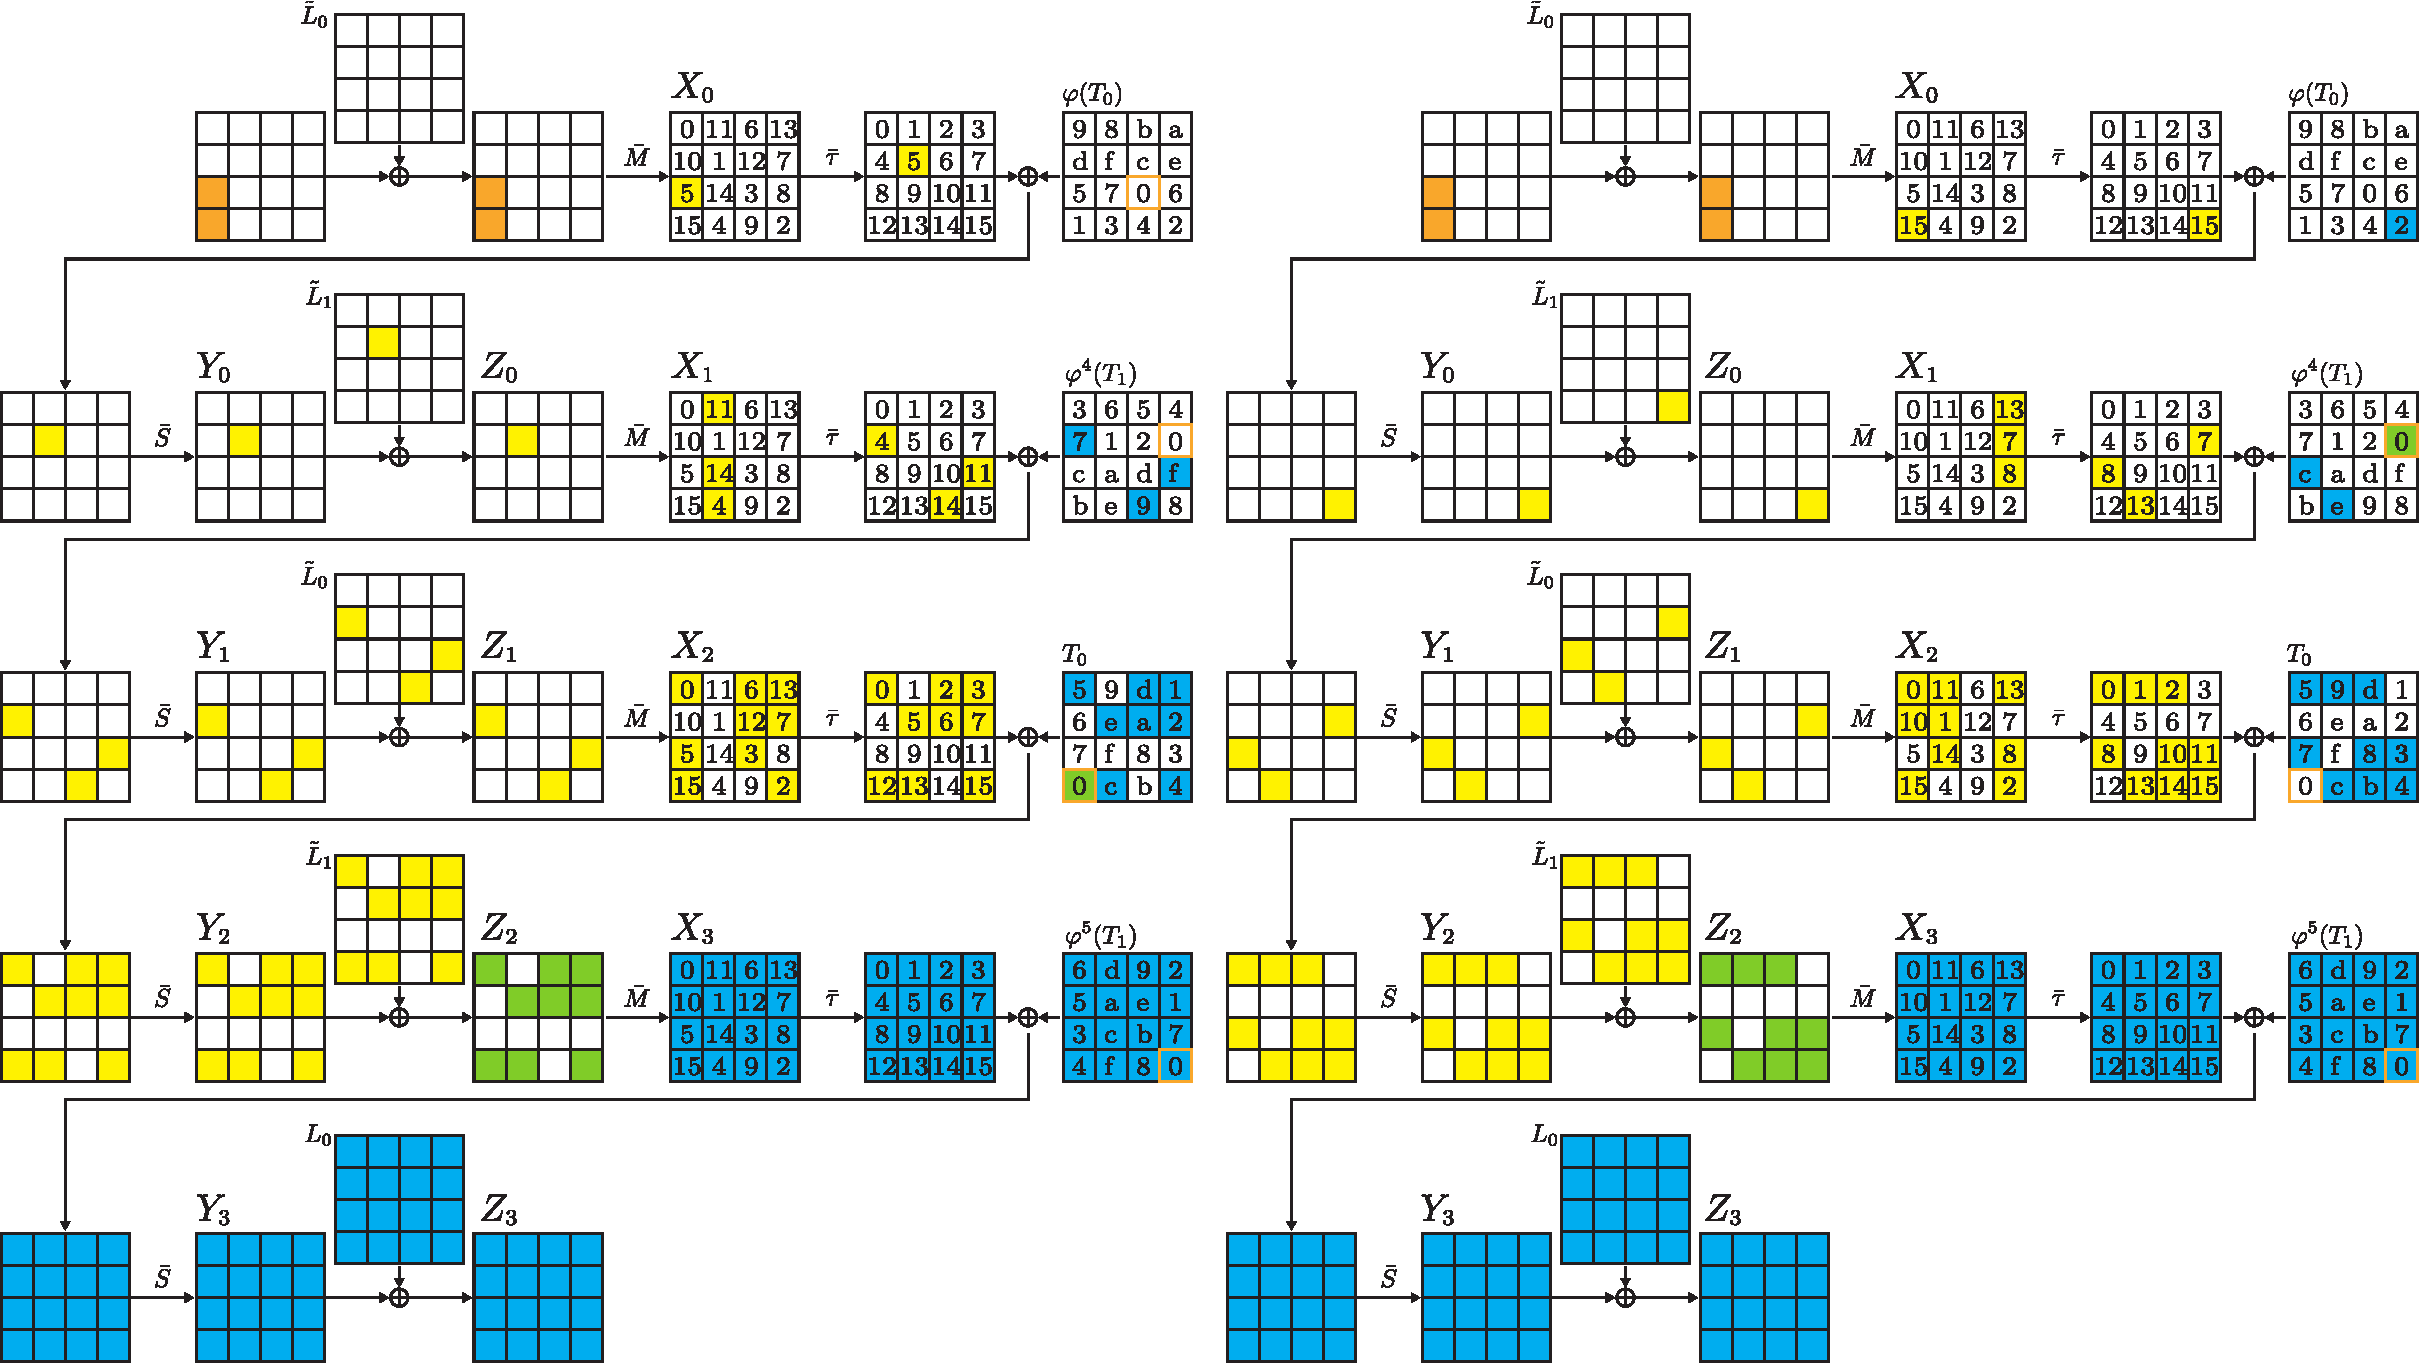
\includegraphics[width=1\textwidth]{./figures/QARMAv2-64-T1-kr.pdf}
\end{center}
\end{columns}
\end{frame}

%%%%%%%%%%%%%%%%%%%%%%%%%%%%%%%%%%%%%%%%%%%%%%%%%%%%%%%%%%%%%%%%%%%%%%%%%%%%%%%
\begin{frame}{Our Key Recovery Attack on \texttt{QARMAv2}-64-128 ($\mathscr{T} = 1$) II}
\vspace{-1cm}
\begin{columns}
\column{0.4\textwidth}
\begin{itemize}
  \scriptsize
  \item Guess $L_{0}$:
  \begin{itemize}
    \scriptsize
    \item Compute $X_{0}[5]$ by partial-sum technique.
    \item Compute $X_{0}[15]$ by partial-sum technique.
    \item Merge the results to derive $2^{64 - 4s}$ candidates for $L_{1}$.
    \item Brute force the remaining $2^{64 - 4s}$ candidates for $L_{1}$ by 1 extra pair.
  \end{itemize}
  \item Each partial-sum involves 36 bits of $L_{1}$.
\end{itemize}
\column{0.6\textwidth}
\begin{center}
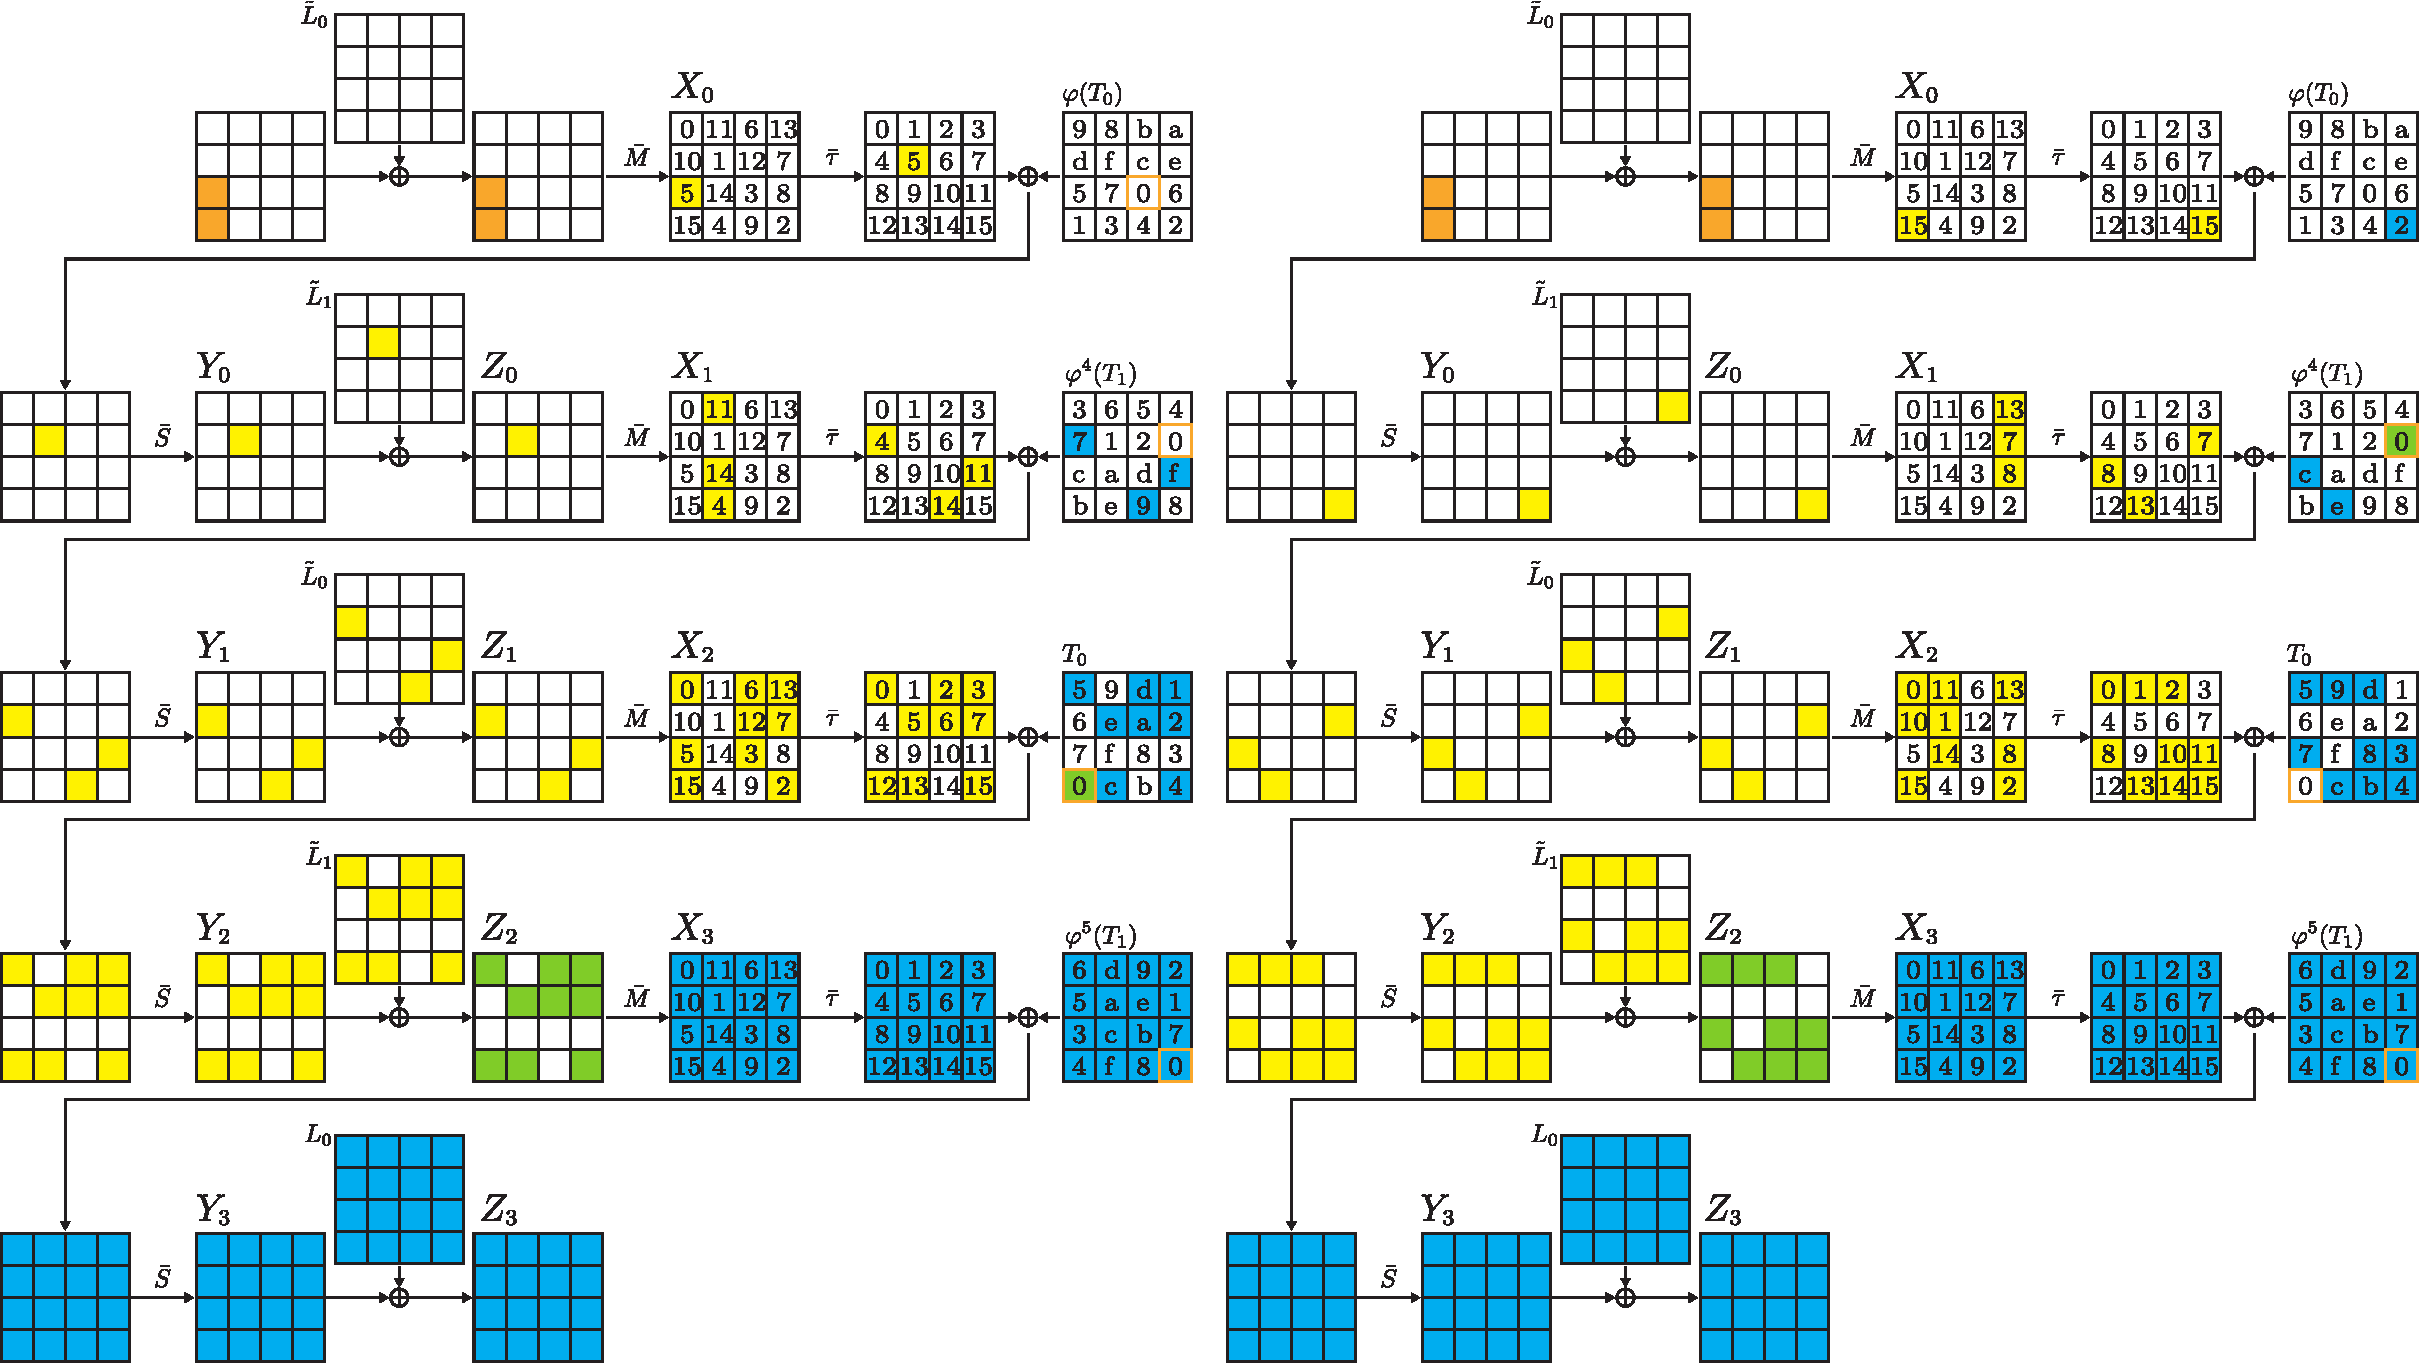
\includegraphics[width=1\textwidth]{./figures/QARMAv2-64-T1-kr.pdf}
\end{center}
\end{columns}
\bgroup\smallmath
\begin{align*}
  &T = 2^{64} \times \left( s \times 2^{44} \mathtt{RF} + s \times 2^{50.15} \mathtt{MA} +  s \times 2^{50.67} \mathtt{MA} + 2^{64 - 4s} \mathtt{ENC} \right)\\
  &\text{For}~ s = 5:~ T = 2^{110.47},~ M = 2^{44},~ D = 5 \times 2^{44}
\end{align*}
\egroup
\end{frame}

%%%%%%%%%%%%%%%%%%%%%%%%%%%%%%%%%%%%%%%%%%%%%%%%%%%%%%%%%%%%%%%%%%%%%%%%%%%%%%%
%%%%%%%%%%%%%%%%%%%%%%%%%%%%%%%%%%%%%%%%%%%%%%%%%%%%%%%%%%%%%%%%%%%%%%%%%%%%%%%
\section{Contributions and Future Works}
\sectionheader[\huge\color{tug}\faHourglassEnd]{Contributions and Future Works}

%%%%%%%%%%%%%%%%%%%%%%%%%%%%%%%%%%%%%%%%%%%%%%%%%%%%%%%%%%%%%%%%%%%%%%%%%%%%%%%

%%%%%%%%%%%%%%%%%%%%%%%%%%%%%%%%%%%%%%%%%%%%%%%%%%%%%%%%%%%%%%%%%%%%%%%%%%%%%%%
\begin{frame}{Contributions and Future Works I}
\begin{table}
  \centering  
  \caption*{Summary of our attacks on \texttt{QARMAv2}. $\mathscr{T}$: No. of independent tweak blocks.}
  \begin{tabular}{lccccc}    
    \toprule
    Version & $\mathscr{T}$ & \#Rounds & Time & Data & Memory\\
    \hline
    \texttt{QARMAv2}-64-128 & 1 & \textbf{13}/16 & $2^{110.47}$ & $2^{46.32}$ & $2^{46.32}$\\
    \midrule    
    \texttt{QARMAv2}-64-128 & 2 & 14/20 & $2^{110.17}$ & $2^{46.32}$ & $2^{46.32}$\\
    \midrule
    \texttt{QARMAv2}-128-256 & 2 & 16/32 & $2^{234.11}$ & $2^{46.58}$ & $2^{46.58}$\\
    \bottomrule
\end{tabular}
\end{table}
\end{frame}

%%%%%%%%%%%%%%%%%%%%%%%%%%%%%%%%%%%%%%%%%%%%%%%%%%%%%%%%%%%%%%%%%%%%%%%%%%%%%%%
\begin{frame}{Contributions and Future Works II}
\vspace{-0.5cm}
\begin{itemize}
\small
\item Contributions
\sparen
\begin{itemize}
\small
\item[\textcolor{tugblue}{\faChevronCircleRight}] Introducing a new CP-based tool to search for integral distinguishers of tweakable block ciphers following the \texttt{TWEAKEY} framework.
\item[\textcolor{tugblue}{\faChevronCircleRight}] Providing the longest concrete key recovery attack against \texttt{QARMAv2}.
\end{itemize}
\item Future works
\sparen
\begin{itemize}
\small
\item[\faRoad] Whether there exists a 12-round integral distinguisher for \texttt{QARMAv2}-128 ($\mathscr{T} = 2$) with data complexity less than $2^{80}$?
\item[\faRoad] Can other cryptanalytic techniques, outperforme our integral attacks, especially for \texttt{QARMAv2}-64-128 ($\mathscr{T} = 1$)? 
\end{itemize} 
\end{itemize}
\begin{center}
\vspace{0.10cm}

% {\large Thanks for your attention!}

% \vspace{0.3cm}
\faGithub: \url{https://github.com/hadipourh/QARMAnalysis}\\
\vspace{0.1cm}
\faArchive: \url{https://ia.cr/2023/1833}
\end{center}
\end{frame}

















%%%%%%%%%%%%%%%%%%%%%%%%%%%%%%%%%%%%%%%%%%%%%%%%%%%%%%%%%%%%%%%%%%%%%%%%%%%%

\begin{frame}[allowframebreaks]{Bibliography}
  \printbibliography
\end{frame}

%%%%%%%%%%%%%%%%%%%%%%%%%%%%%%%%%%%%%%%%%%%%%%%%%%%%%%%%%%%%%%%%%%%%%%%%%%%%

%%%%%%%%%%%%%%%%%%%%%%%%%%%%%%%%%%%%%%%%%%%%%%%%%%%%%%%%%%%%%%%%%%%%%%%%%%%%
% Backup slides

\begin{frame}{14-Round Integral Attack on \texttt{QARMAv2}-64-128 ($\mathscr{T} = 2$)}
\vspace{-1cm}
\begin{columns}
\column{0.3\textwidth}
\begin{figure}
\centering
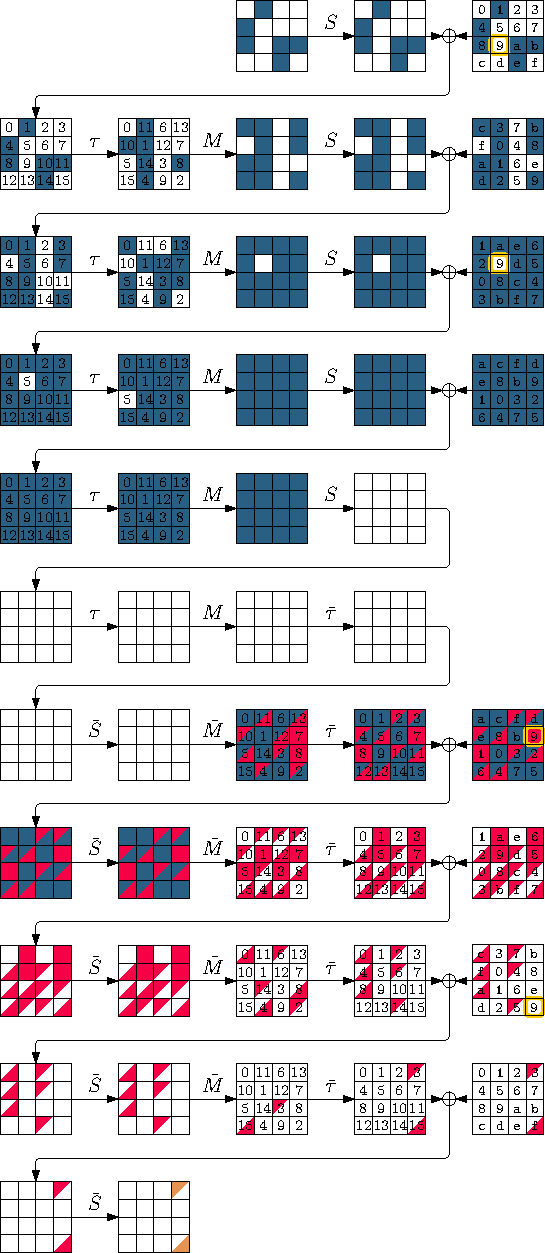
\includegraphics[width=0.6\textwidth]{./figures/qarmav2_64_t2_10r_v0.pdf}
\end{figure}

\column{0.7\textwidth}
\begin{figure}
\centering
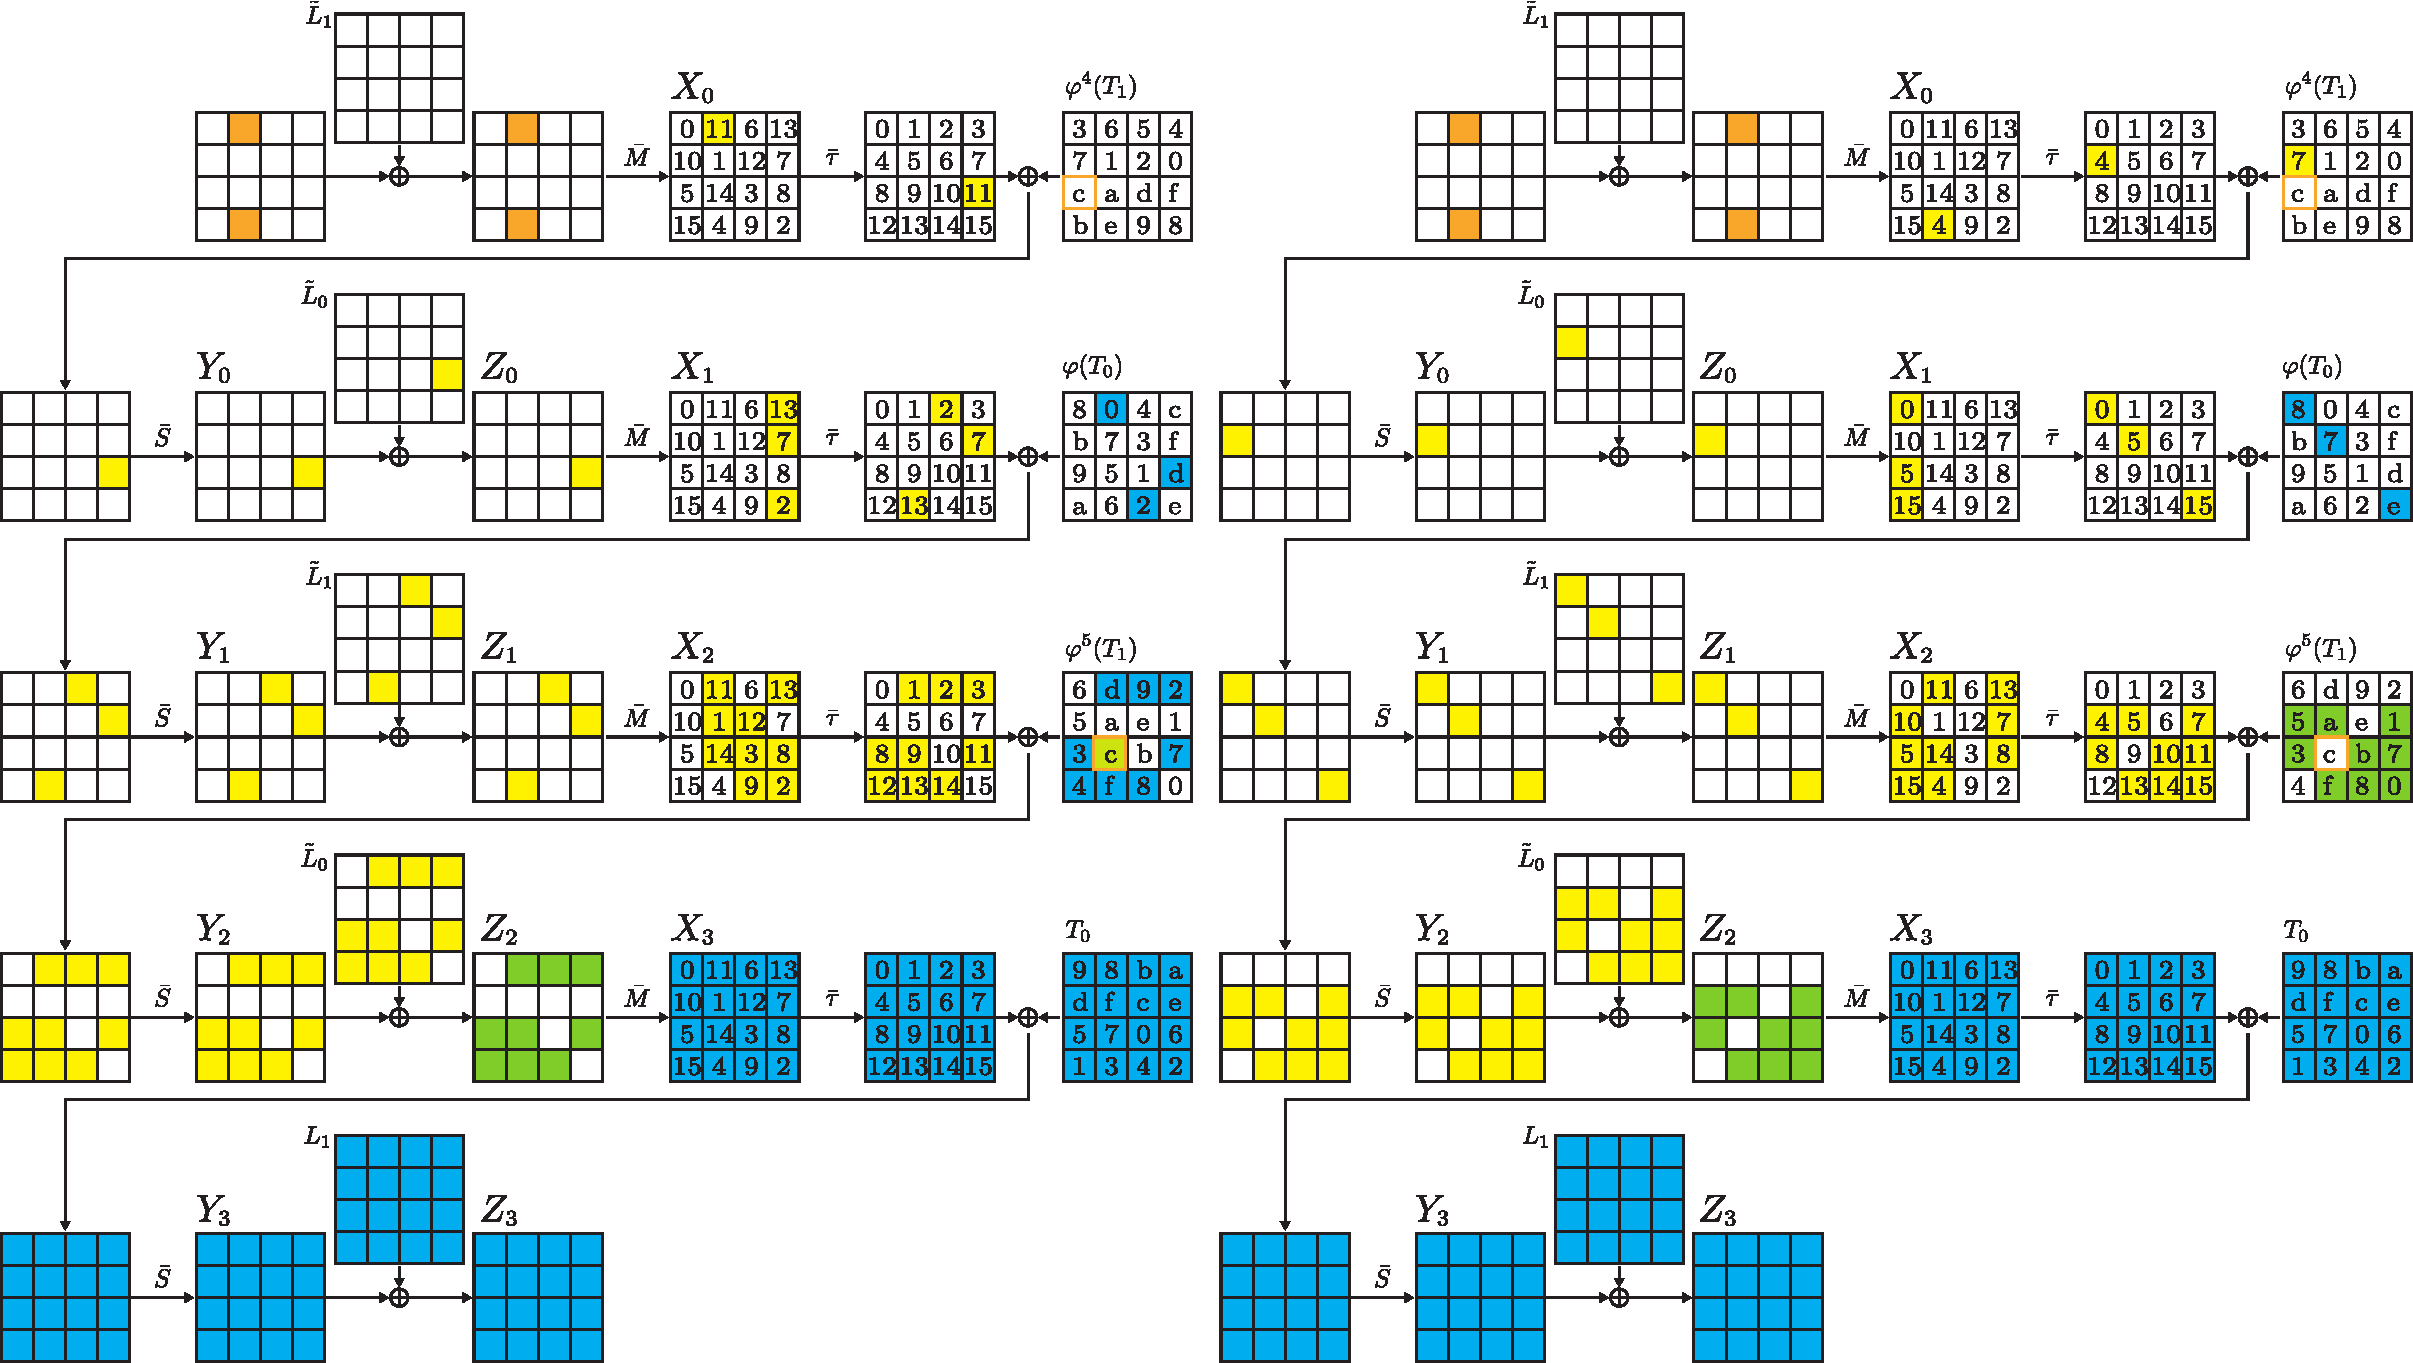
\includegraphics[width=0.85\textwidth]{figures/QARMAv2-64-T2-kr.pdf}
\end{figure}
\end{columns}
\end{frame}

%%%%%%%%%%%%%%%%%%%%%%%%%%%%%%%%%%%%%%%%%%%%%%%%%%%%%%%%%%%%%%%%%%%%%%%%%%%%
\begin{frame}{16-Round Integral Attack on \texttt{QARMAv2}-128-256 ($\mathscr{T} = 2$)}
\vspace{-1.2cm}
\begin{columns}
\column{0.3\textwidth}
\begin{figure}
\centering
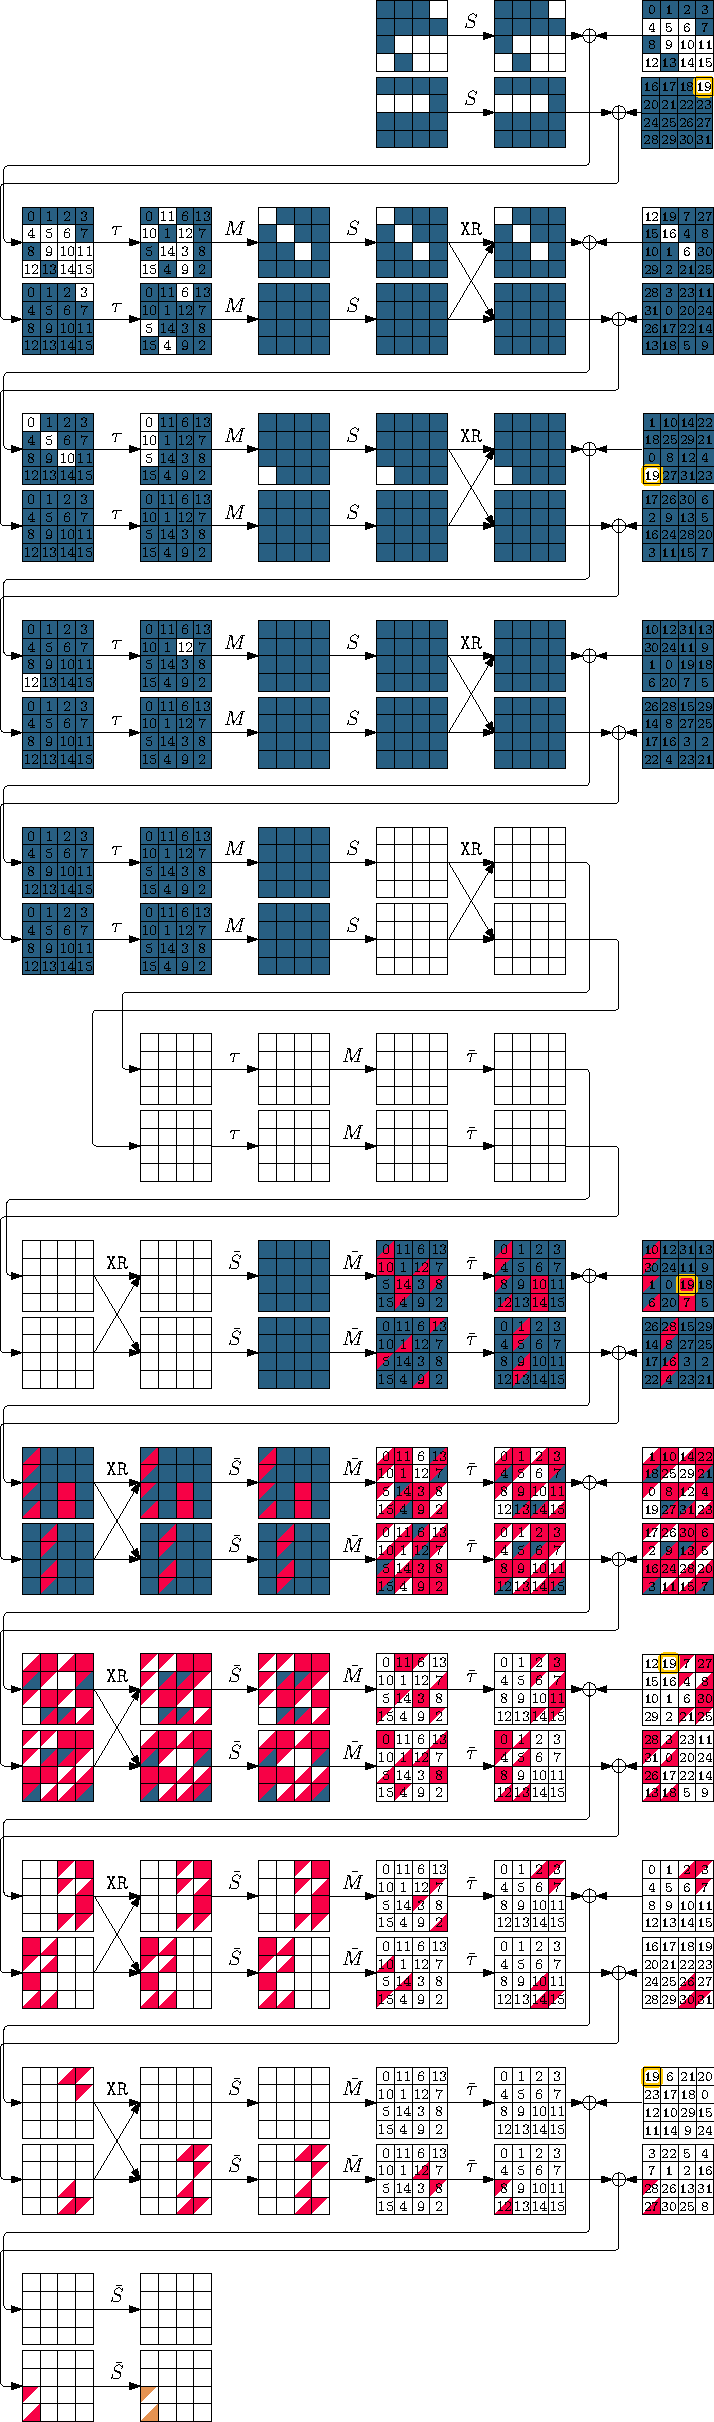
\includegraphics[width=0.43\textwidth]{./figures/qarmav2_128_t2_11r_v1.pdf}
\end{figure}

\column{0.7\textwidth}
\begin{figure}
\centering
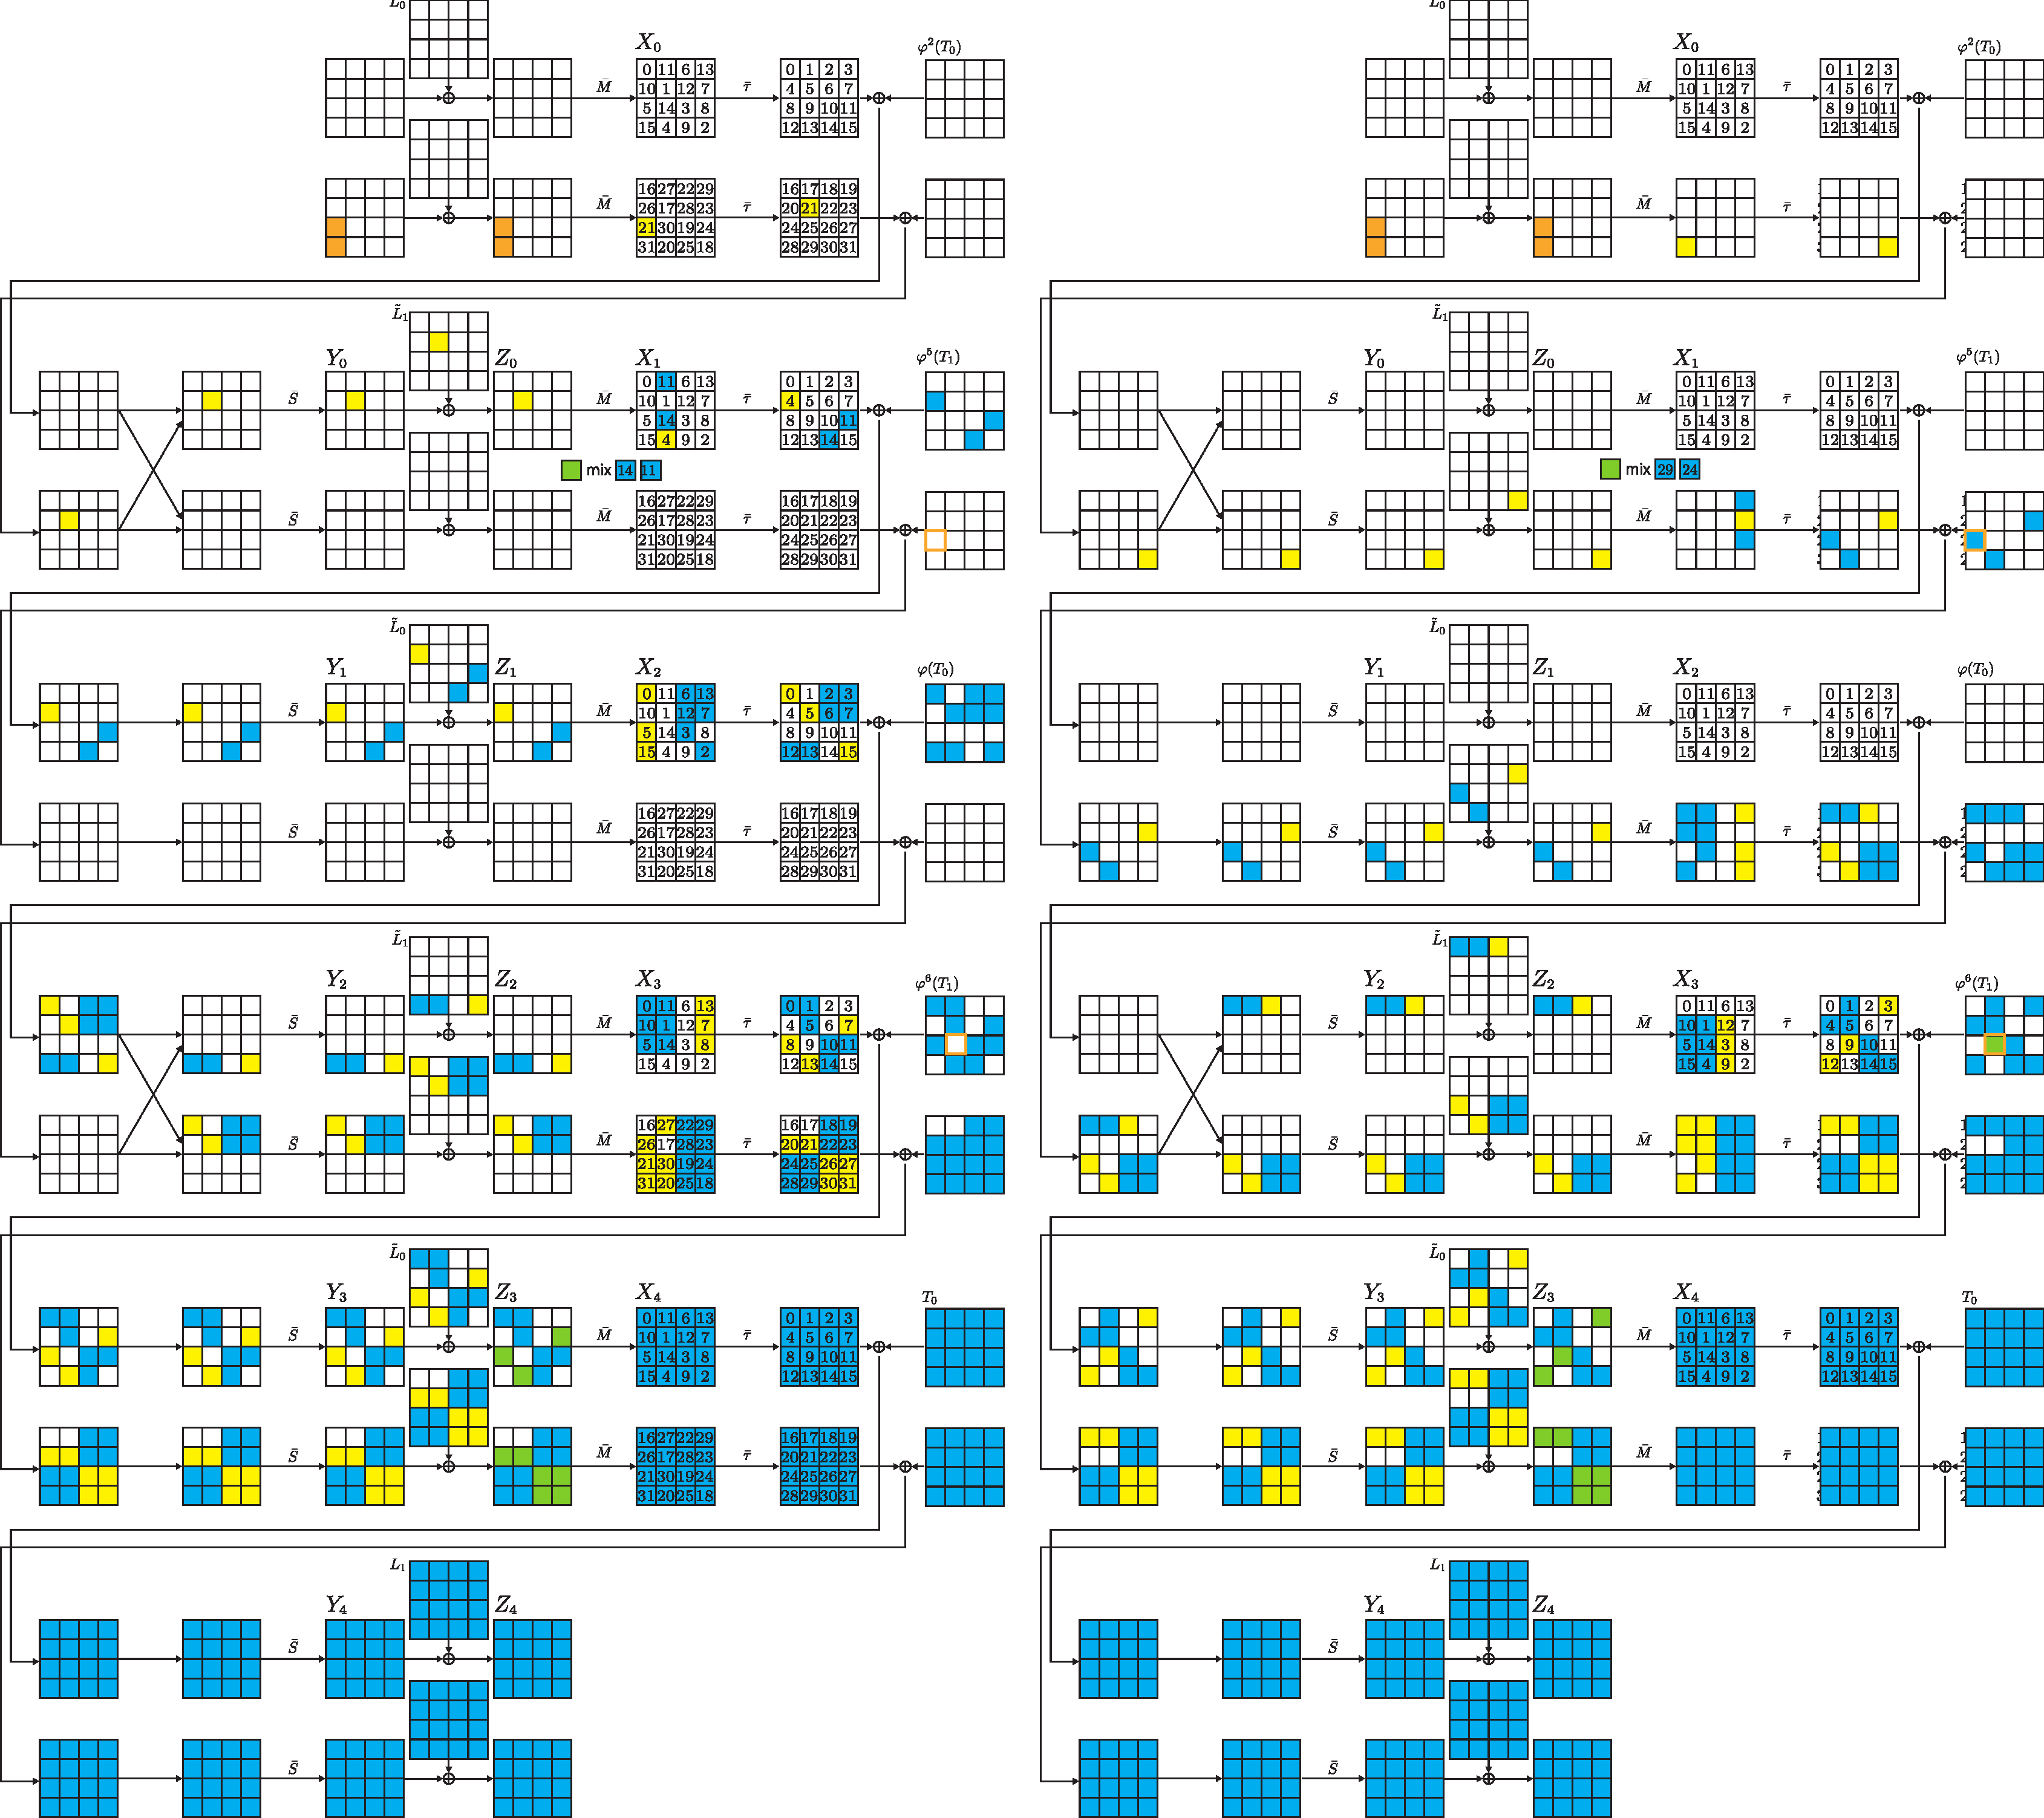
\includegraphics[width=0.65\textwidth]{./figures/QARMAv2-128-kr.pdf}
\end{figure}
\end{columns}
\end{frame}

%%%%%%%%%%%%%%%%%%%%%%%%%%%%%%%%%%%%%%%%%%%%%%%%%%%%%%%%%%%%%%%%%%%%%%%%%%%%

\begin{filecontents*}[overwrite]{\jobname.bib}
% impossible differential Biham (miss-in-the-middle technique)
@inproceedings{eurocrypt_BihamBS99,
  author    = {Eli Biham and
                Alex Biryukov and
                Adi Shamir},
  title     = {Cryptanalysis of Skipjack Reduced to 31 Rounds Using Impossible Differentials},
  booktitle = {{EUROCRYPT} 1999},
  series    = {LNCS},
  volume    = {1592},
  pages     = {12--23},
  publisher = {Springer},
  year      = {1999},
  doi       = {10.1007/3-540-48910-X_2}
}

% impossible differential Knudesen
@article{knudsen1998deal,
  title     = {DEAL-a 128-bit block cipher},
  author    = {Knudsen, Lars},
  journal   = {complexity},
  volume    = {258},
  number    = {2},
  pages     = {216},
  year      = {1998},
  publisher = {Citeseer}
}

% milp-based method to search for ID attacks - works for ARX and SPN
@misc{eprint_Cui,
  author    = {Tingting Cui and 
            Shiyao Chen and 
            Keting Jia and 
            Kai Fu and 
            Meiqin Wang},
  title     = {New Automatic Search Tool for Impossible Differentials and Zero-Correlation Linear Approximations},
  howpublished = {IACR Cryptology ePrint Archive, Report 2016/689},
  year      = {2016},
  url       = {https://eprint.iacr.org/2016/689}
}

% milp-based method to search for ID attacks - works for SPN
@inproceedings{eurocrypt_SasakiTodo2017,
  author    = {Sasaki, Yu and 
                Todo, Yosuke},              
  Xeditor    = {Coron, Jean-S{\'e}bastien
                and 
                Nielsen, Jesper Buus},
  title     = {New Impossible Differential Search Tool from Design and Cryptanalysis Aspects},
  Xbooktitle = {Advances in Cryptology -- EUROCRYPT 2017},
  booktitle = {{EUROCRYPT} 2017},
  year      = {2017},
  publisher = {Springer International Publishing},
  address   = {Cham},
  pages     = {185--215},
  doi       = {10.1007/978-3-319-56617-7_7}
}

% cp-based method by sun and gerault
@article{tosc_SunGLYTQH2017,
author      = {Sun, Siwei and 
            Gerault, David and 
            Lafourcade, Pascal and 
            Yang, Qianqian and 
            Todo, Yosuke and 
            Qiao, Kexin and 
            Hu, Lei}, 
  title     = {Analysis of {AES}, {SKINNY}, and Others with Constraint Programming}, 
  volume    = {2017}, 
  doi       = {10.13154/tosc.v2017.i1.281-306}, 
  number    = {1}, 
  journal   = {IACR Transactions on Symmetric Cryptology}, 
  year      = {2017}, 
  month     = {Mar.}, 
  pages     = {281–306} 
}

% patrick's tool for mitm and id attacks
@inproceedings{crypto_DerbezF16,
  author    = {Patrick Derbez and
                Pierre-Alain Fouque},
  title     = {Automatic Search of Meet-in-the-Middle and Impossible Differential
                Attacks},
  booktitle = {{CRYPTO} 2016},
  series    = {LNCS},
  volume    = {9815},
  pages     = {157--184},
  publisher = {Springer},
  year      = {2016}
}

% milp model of division 
@inproceedings{asiacrypt_XiangZBL16,
  author    = {Zejun Xiang and
                Wentao Zhang and
                Zhenzhen Bao and
                Dongdai Lin},
  title     = {Applying {MILP} Method to Searching Integral Distinguishers Based
                on Division Property for 6 Lightweight Block Ciphers},
  booktitle = {{ASIACRYPT} 2016},
  series    = {LNCS},
  volume    = {10031},
  pages     = {648--678},
  year      = {2016},
  doi       = {10.1007/978-3-662-53887-6_24}
}

% cp model to encode the deterministic truncated trails
@article{tosc_SunGWW2020, 
  author    = {Sun, Ling and Gerault, David and Wang, Wei and Wang, Meiqin},
  title     = {On the Usage of Deterministic (Related-Key) Truncated Differentials and Multidimensional Linear Approximations for SPN Ciphers}, 
  volume    = {2020},   
  doi       = {10.13154/tosc.v2020.i3.262-287}, 
  number    = {3}, 
  journal   = {IACR Transactions on Symmetric Cryptology}, 
  year      = {2020}, 
  month     = {Sep.}, 
  pages     = {262–287}
}

% blns2018
@article{joc_BouraLNS2018,
  author    = {Boura, Christina and 
                Lallemand, Virginie and 
                Naya-Plasencia, Mar{\'\i}a and 
                Suder, Valentin},
  title     = {Making the impossible possible},
  journal   = {Journal of Cryptology},
  volume    = {31},
  number    = {1},
  pages     = {101--133},
  year      = {2018},
  publisher = {Springer},
  doi       = {10.1007/s00145-016-9251-7}
}

% bns2014
@inproceedings{asiacrypt_BouraNS2014,
  author    = {Boura, Christina and 
                Naya-Plasencia, Maria and 
                Suder, Valentin},
  title     = {Scrutinizing and improving impossible differential attacks: applications to CLEFIA, Camellia, LBlock and Simon},
  booktitle = {International Conference on the Theory and Application of Cryptology and Information Security},
  pages     = {179--199},
  year      = {2014},
  organization = {Springer},
  doi       = {10.1007/978-3-662-45611-8_10}
}

% MiniZinc
@inproceedings{cp_NethercoteSBBDT07,
  author    = {Nicholas Nethercote and
                Peter J. Stuckey and
                Ralph Becket and
                Sebastian Brand and
                Gregory J. Duck and
                Guido Tack},
  title     = {MiniZinc: Towards a Standard {CP} Modelling Language},
  booktitle = {{CP} 2007},
  series    = {LNCS},
  volume    = {4741},
  pages     = {529--543},
  publisher = {Springer},
  year      = {2007}
}

@misc{gurobi,
  author    = {{Gurobi Optimization, LLC}},
  title     = {{Gurobi Optimizer Reference Manual}},
  year      = {2022},
  url       = {https://www.gurobi.com}
}

% Or-Tools
@software{ortools,
  author    = {Laurent Perron and Vincent Furnon},
  title     = {{OR-Tools}},
  version   = {9.3},
  organization = {Google},
  url       = {https://developers.google.com/optimization/},
  date      = {2022-3-15}
}

% seminal paper of ZC attack
@article{dcc_BogdanovR14,
  author    = {Andrey Bogdanov and
                Vincent Rijmen},
  title     = {Linear hulls with correlation zero and linear cryptanalysis of block
                ciphers},
  journal   = {Des. Codes Cryptogr.},
  volume    = {70},
  number    = {3},
  pages     = {369--383},
  year      = {2014},
  doi       = {10.1007/s10623-012-9697-z}
}

% multidimensional zc and link between zc and integral attacks
@inproceedings{asiacrypt_BogdanovLNW12,
  author    = {Andrey Bogdanov and
                Gregor Leander and
                Kaisa Nyberg and
                Meiqin Wang},
  title     = {Integral and Multidimensional Linear Distinguishers with Correlation
                Zero},
  booktitle = {{ASIACRYPT} 2012},
  series    = {LNCS},
  volume    = {7658},
  pages     = {244--261},
  publisher = {Springer},
  year      = {2012},
  doi       = {10.1007/978-3-642-34961-4_16}
}

% link between ZC, ID and Integral attacks
@inproceedings{crypto_SunLRLCWAL15,
  author    = {Bing Sun and
                Zhiqiang Liu and
                Vincent Rijmen and
                Ruilin Li and
                Lei Cheng and
                Qingju Wang and
                Hoda AlKhzaimi and
                Chao Li},
  title     = {Links Among Impossible Differential, Integral and Zero Correlation
                Linear Cryptanalysis},
  booktitle = {{CRYPTO} 2015},
  series    = {LNCS},
  volume    = {9215},
  pages     = {95--115},
  publisher = {Springer},
  year      = {2015},
  doi       = {10.1007/978-3-662-47989-6_5}
}

% zc-integral attack
@article{tosc_AnkeleDGLGY2019, 
  author    = {Ankele, Ralph and Dobraunig, Christoph and Guo, Jian and Lambooij, Eran and Leander, Gregor and Todo, Yosuke}, 
  title     = {Zero-Correlation Attacks on Tweakable Block Ciphers with Linear Tweakey Expansion}, 
  volume    = {2019},
  doi       = {10.13154/tosc.v2019.i1.192-235}, 
  number    = {1}, 
  journal   = {IACR Transactions on Symmetric Cryptology}, 
  year      = {2019},
  month     = {Mar.}, 
  pages     = {192–235},
}

% ID-RT and ZC-ST attacks on SKINNY (Sadeghi et al.)
@article{tosc_SadeghiMB18,
  author    = {Sadegh Sadeghi and
                Tahereh Mohammadi and
                Nasour Bagheri},
  title     = {Cryptanalysis of Reduced round {SKINNY} Block Cipher},
  journal   = {{IACR} Trans. Symmetric Cryptol.},
  volume    = {2018},
  number    = {3},
  pages     = {124--162},
  year      = {2018},
  doi       = {10.13154/tosc.v2018.i3.124-162}
}

% ID attacks on SKINNY in the ST setting (IET)
@article{iet_YangQC17,
  author    = {Dong Yang and
                Wen{-}Feng Qi and
                Hua{-}Jin Chen},
  title     = {Impossible differential attacks on the {SKINNY} family of block ciphers},
  journal   = {{IET} Inf. Secur.},
  volume    = {11},
  number    = {6},
  pages     = {377--385},
  year      = {2017},
  doi       = {10.1049/iet-ifs.2016.0488}
}

% ID attack on SKINNY in the RT setting (ToSC)
@article{journals_tosc_LiuGL17,
  author    = {Guozhen Liu and
                Mohona Ghosh and
                Ling Song},
  title     = {Security Analysis of {SKINNY} under Related-Tweakey Settings},
  journal   = {{IACR} Trans. Symmetric Cryptol.},
  volume    = {2017},
  number    = {3},
  pages     = {37--72},
  year      = {2017},
  doi       = {10.13154/tosc.v2017.i3.37-72}
}

% ID attack on SKINNY (Tolba) WRONG RESULTS!
@inproceedings{africacrypt_Tolba0Y17,
  author    = {Mohamed Tolba and
                Ahmed Abdelkhalek and
                Amr M. Youssef},
  title     = {Impossible Differential Cryptanalysis of Reduced-Round {SKINNY}},
  booktitle = {{AFRICACRYPT} 2017},
  series    = {LNCS},
  volume    = {10239},
  pages     = {117--134},
  year      = {2017},
  doi       = {10.1007/978-3-319-57339-7_7}
}

@article{Zhang2022,
  author    = {Zhang, Yi and
                Cui, Ting and
                Wang, Congjun},
  title     = {{Zero-correlation} linear attack on reduced-round {SKINNY}},
  journal   = {Frontiers of Computer Science},
  volume    = {17},
  number    = {174808 (2023)},
  pages     = {377--385},
  year      = {2022},
  doi       = {10.1007/s11704-022-2206-2}
}

% skinny specification
@inproceedings{skinny,  
  author    = {Beierle, Christof and 
              Jean, J{\'e}r{\'e}my and 
              K{\"o}lbl, Stefan and 
              Leander, Gregor and 
              Moradi, Amir and 
              Peyrin, Thomas and 
              Sasaki, Yu and 
              Sasdrich, Pascal and 
              Sim, Siang Meng},
  title     = {{The SKINNY family of block ciphers and its low-latency variant MANTIS}},
  Xbooktitle= {Advances in Cryptology -- CRYPTO 2016},
  booktitle = {{CRYPTO} 2016},
  pages     = {123--153},
  year      = {2016},
  organization= {Springer},
  doi       = {10.1007/978-3-662-53008-5_5},
}

% QARMAv2 block cipher
@article{cryptoeprint_qarmav2,
  author       = {Roberto Avanzi and
                  Subhadeep Banik and
                  Orr Dunkelman and
                  Maria Eichlseder and
                  Shibam Ghosh and
                  Marcel Nageler and
                  Francesco Regazzoni},
  title        = {The {QARMAv2} Family of Tweakable Block Ciphers},
  journal      = {{IACR} Trans. Symmetric Cryptol.},
  volume       = {2023},
  number       = {3},
  pages        = {25--73},
  year         = {2023},
  doi          = {10.46586/TOSC.V2023.I3.25-73},
}

% related key zc/integral
@inproceedings{ctrsa_NiuLSW21,
  author    = {Chao Niu and
                Muzhou Li and
                Siwei Sun and
                Meiqin Wang},
  title     = {Zero-Correlation Linear Cryptanalysis with Equal Treatment for Plaintexts
                and Tweakeys},
  booktitle = {{CT-RSA} 2021},
  series    = {LNCS},
  volume    = {12704},
  pages     = {126--147},
  publisher = {Springer},
  year      = {2021},
  doi       = {10.1007/978-3-030-75539-3_6}
}

% Our EUROCRYPT 2023 paper
@inproceedings{eurocrypt_HadipourSE23,
  author       = {Hosein Hadipour and
                  Sadegh Sadeghi and
                  Maria Eichlseder},
  title        = {Finding the Impossible: Automated Search for Full Impossible Differential,
                  Zero-Correlation, and Integral Attacks},
  booktitle    = {{EUROCRYPT} 2023},
  series       = {LNCS},
  volume       = {14007},
  pages        = {128--157},
  publisher    = {Springer},
  year         = {2023},
  doi          = {10.1007/978-3-031-30634-1_5}
}

% ForkCipher Cryptanalysis
@article{tosc_BariantDL20,
  author       = {Augustin Bariant and
                  Nicolas David and
                  Ga{\"{e}}tan Leurent},
  title        = {Cryptanalysis of {Forkciphers}},
  journal      = {{IACR} Trans. Symmetric Cryptol.},
  volume       = {2020},
  number       = {1},
  pages        = {233--265},
  year         = {2020},
  doi          = {10.13154/tosc.v2020.i1.233-265}
}

% One of the seminal papers for integral attacks
@incollection{hod_discrete_derivatives_lai1994higher,
  author    = {Lai, Xuejia},
  title     = {Higher order derivatives and differential cryptanalysis},
  booktitle = {Communications and cryptography},
  pages     = {227--233},
  year      = {1994},
  publisher = {Springer}
}

% One of the seminal papers for integral attacks
@inproceedings{square_fse_DaemenKR97,
  author    = {Joan Daemen and
                Lars R. Knudsen and
                Vincent Rijmen},
  title     = {The Block Cipher {Square}},
  booktitle = {{FSE} 1997},
  series    = {LNCS},
  volume    = {1267},
  pages     = {149--165},
  publisher = {Springer},
  year      = {1997},
  doi       = {10.1007/BFb0052343},
}

% the early abort tehnique
@inproceedings{ctrsa_LuKKD08,
  author    = {Jiqiang Lu and
                Jongsung Kim and
                Nathan Keller and
                Orr Dunkelman},
  title     = {Improving the Efficiency of Impossible Differential Cryptanalysis
                of Reduced {Camellia} and {MISTY1}},
  booktitle = {{CT-RSA} 2008},
  series    = {LNCS},
  volume    = {4964},
  pages     = {370--386},
  publisher = {Springer},
  year      = {2008},
  doi          = {10.1007/978-3-540-79263-5_24},
}

% partial sum technique
@inproceedings{fseFergusonKLSSWW00,
  author    = {Niels Ferguson and
                John Kelsey and
                Stefan Lucks and
                Bruce Schneier and
                Michael Stay and
                David A. Wagner and
                Doug Whiting},
  Xeditor   = {Bruce Schneier},
  title     = {Improved Cryptanalysis of {Rijndael}},
  booktitle = {{FSE} 2000},
  series    = {LNCS},
  volume    = {1978},
  pages     = {213--230},
  publisher = {Springer},
  year      = {2000},
  doi       = {10.1007/3-540-44706-7_15},
}

% The seminal paper for undisrupted bits
@article{journals_jcam_Tezcan14_ubits,
  author       = {Cihangir Tezcan},
  title        = {Improbable differential attacks on {Present} using undisturbed bits},
  journal      = {J. Comput. Appl. Math.},
  volume       = {259},
  pages        = {503--511},
  year         = {2014},
  doi          = {10.1016/j.cam.2013.06.023}
}

% MitM in integral key recovery
@inproceedings{sacryptSasaki012,
  author    = {Yu Sasaki and
               Lei Wang},
  title     = {Meet-in-the-Middle Technique for Integral Attacks against {Feistel}
               Ciphers},
  booktitle = {SAC 2012},
  series    = {LNCS},
  volume    = {7707},
  pages     = {234--251},
  publisher = {Springer},
  year      = {2012},
  doi       = {10.1007/978-3-642-35999-6_16},
}

  
\end{filecontents*}

\end{document}
